\documentclass[a4paper]{article}



%% Language and font encodings
\usepackage[english]{babel}
\usepackage[utf8]{inputenc}
\usepackage[T1]{fontenc}

%% Sets page size and margins
\usepackage[a4paper,top=2.5cm,bottom=2.5cm,left=2.5cm,right=2.5cm,marginparwidth=1.75cm]{geometry}

%% Useful packages
\usepackage{paralist}
\usepackage{amsmath}
\usepackage{bbm}
\usepackage{amsthm}
\usepackage{graphicx}
\usepackage[colorinlistoftodos]{todonotes}
\usepackage[colorlinks=true, allcolors=blue]{hyperref}
\usepackage{nameref,cleveref}
\usepackage{tikz}
% tikzlibrary.code.tex
%
% Copyright 2010-2011 by Laura Dietz
% Copyright 2012 by Jaakko Luttinen
%
% The MIT License
%
% See LICENSE file for more details.

% Load other libraries
\usetikzlibrary{shapes}
\usetikzlibrary{fit}
\usetikzlibrary{chains}
\usetikzlibrary{arrows}

% Latent node
\tikzstyle{latent} = [circle,fill=white,draw=black,inner sep=1pt,
minimum size=20pt, font=\fontsize{10}{10}\selectfont, node distance=1]
% Observed node
\tikzstyle{obs} = [latent,fill=gray!25]
% Constant node
\tikzstyle{const} = [rectangle, inner sep=0pt, node distance=1]
% Factor node
\tikzstyle{factor} = [rectangle, fill=black,minimum size=5pt, inner
sep=0pt, node distance=0.4]
% Deterministic node
\tikzstyle{det} = [latent, diamond]

% Plate node
\tikzstyle{plate} = [draw, rectangle, rounded corners, fit=#1]
% Invisible wrapper node
\tikzstyle{wrap} = [inner sep=0pt, fit=#1]
% Gate
\tikzstyle{gate} = [draw, rectangle, dashed, fit=#1]

% Caption node
\tikzstyle{caption} = [font=\footnotesize, node distance=0] %
\tikzstyle{plate caption} = [caption, node distance=0, inner sep=0pt,
below left=5pt and 0pt of #1.south east] %
\tikzstyle{factor caption} = [caption] %
\tikzstyle{every label} += [caption] %

%\pgfdeclarelayer{b}
%\pgfdeclarelayer{f}
%\pgfsetlayers{b,main,f}

% \factoredge [options] {inputs} {factors} {outputs}
\newcommand{\factoredge}[4][]{ %
  % Connect all nodes #2 to all nodes #4 via all factors #3.
  \foreach \f in {#3} { %
    \foreach \x in {#2} { %
      \path (\x) edge[-,#1] (\f) ; %
      %\draw[-,#1] (\x) edge[-] (\f) ; %
    } ;
    \foreach \y in {#4} { %
      \path (\f) edge[->, >={triangle 45}, #1] (\y) ; %
      %\draw[->,#1] (\f) -- (\y) ; %
    } ;
  } ;
}

% \edge [options] {inputs} {outputs}
\newcommand{\edge}[3][]{ %
  % Connect all nodes #2 to all nodes #3.
  \foreach \x in {#2} { %
    \foreach \y in {#3} { %
      \path (\x) edge [->, >={triangle 45}, #1] (\y) ;%
      %\draw[->,#1] (\x) -- (\y) ;%
    } ;
  } ;
}

% \factor [options] {name} {caption} {inputs} {outputs}
\newcommand{\factor}[5][]{ %
  % Draw the factor node. Use alias to allow empty names.
  \node[factor, label={[name=#2-caption]#3}, name=#2, #1,
  alias=#2-alias] {} ; %
  % Connect all inputs to outputs via this factor
  \factoredge {#4} {#2-alias} {#5} ; %
}

% \plate [options] {name} {fitlist} {caption}
\newcommand{\plate}[4][]{ %
  \node[wrap=#3] (#2-wrap) {}; %
  \node[plate caption=#2-wrap] (#2-caption) {#4}; %
  \node[plate=(#2-wrap)(#2-caption), #1] (#2) {}; %
}

% \gate [options] {name} {fitlist} {inputs}
\newcommand{\gate}[4][]{ %
  \node[gate=#3, name=#2, #1, alias=#2-alias] {}; %
  \foreach \x in {#4} { %
    \draw [-*,thick] (\x) -- (#2-alias); %
  } ;%
}

% \vgate {name} {fitlist-left} {caption-left} {fitlist-right}
% {caption-right} {inputs}
\newcommand{\vgate}[6]{ %
  % Wrap the left and right parts
  \node[wrap=#2] (#1-left) {}; %
  \node[wrap=#4] (#1-right) {}; %
  % Draw the gate
  \node[gate=(#1-left)(#1-right)] (#1) {}; %
  % Add captions
  \node[caption, below left=of #1.north ] (#1-left-caption)
  {#3}; %
  \node[caption, below right=of #1.north ] (#1-right-caption)
  {#5}; %
  % Draw middle separation
  \draw [-, dashed] (#1.north) -- (#1.south); %
  % Draw inputs
  \foreach \x in {#6} { %
    \draw [-*,thick] (\x) -- (#1); %
  } ;%
}

% \hgate {name} {fitlist-top} {caption-top} {fitlist-bottom}
% {caption-bottom} {inputs}
\newcommand{\hgate}[6]{ %
  % Wrap the left and right parts
  \node[wrap=#2] (#1-top) {}; %
  \node[wrap=#4] (#1-bottom) {}; %
  % Draw the gate
  \node[gate=(#1-top)(#1-bottom)] (#1) {}; %
  % Add captions
  \node[caption, above right=of #1.west ] (#1-top-caption)
  {#3}; %
  \node[caption, below right=of #1.west ] (#1-bottom-caption)
  {#5}; %
  % Draw middle separation
  \draw [-, dashed] (#1.west) -- (#1.east); %
  % Draw inputs
  \foreach \x in {#6} { %
    \draw [-*,thick] (\x) -- (#1); %
  } ;%
}

\usetikzlibrary{datavisualization}
\usetikzlibrary{datavisualization.formats.functions}
\newcommand{\fixgmfont}[1]{\scalebox{0.8}{#1}}

\usepackage{../includes/MarkMathCmds}
\usepackage{mathtools}
\newcommand{\mat}[1]{{\boldsymbol{{#1}}}} % matrix

\usepackage{../includes/MarkBiblatexCmds}
\addbibresource{../includes/pi-literature.bib}


\newcommand{\mx}{\vm_\vx}
\newcommand{\my}{\vm_\vy}
\newcommand{\covmat}{\boldsymbol{\Sigma}}
\newcommand{\covx}{\boldsymbol{\Sigma}_{\vx\vx}}
\newcommand{\covy}{\boldsymbol{\Sigma}_{\vy\vy}}
\newcommand{\covxy}{\boldsymbol{\Sigma}_{\vx\vy}}
\newcommand{\covyx}{\boldsymbol{\Sigma}_{\vy\vx}}

\newcommand{\K}{\mathbf{K}}

\newcommand{\questionref}[1]{\Cref{#1} -- \nameref{#1}}

\newcommand{\lb}{\mathcal{L}}
\newcommand{\sumn}{\sum_{n=1}^N}

\theoremstyle{definition}
\newtheorem{question}{Question}


\title{70019 Probabilistic Inference: Study Guide}
\author{Mark van der Wilk\footnote{Many thanks to teaching assistants Anish Dhir, Seth Nabarro, and Filippo Valdettaro for their improvements to the document.} \\ \texttt{m.vdwilk@imperial.ac.uk}}




\begin{document}
\maketitle


\section{Overview}
This document will provide:
\begin{itemize}
\item references to some prerequisites and useful background material,
\item clarification on notation conventions used in the course,
\item some useful identities (some of these assumed knowledge in the exam),
\item exercises and their answers.
\end{itemize}
This document will be continuously updated during the course with more exercises, pointers and identities. Please e-mail me about any errors or comments.


\section{Background material}
You will be expected to have a \emph{firm} understanding of Mathematics for Machine Learning. In the explanations, I will be manipulating probabilities and expectations freely, as discussed in Mathematics for Machine Learning. If steps are difficult, I encourage you to raise this on the course EdStem page, or during a Q\&A session.

\begin{itemize}
\item Basic probability: sample spaces, disjoint events (summation of probabilities), independent events (multiplication of probabilities). See \citet{walpole2012probability}, Ch2 (Imperial Library, or search Google for reading options).
\item Probability densities. See \citet{mml} \S 6.2.
\item Sum, product \& Bayes' rules. See \citet{mml} \S 6.3.
\item Unconstrained continuous optimisation. See \citet{mml} \S 7.1.
\item Linear algebra and matrix decompositions. See \citet{mml} ch 4 (and Chs 2 and 3 for basics).
\item A familiarity with linear basis-function regression. See \citet{mml} ch 9.
\end{itemize}


\section{Notation of probabilities}
In this course we will use the notation for probabilities that is common in machine learning. The main advantage is that this notation is shorter, although it does leave certain things implicit.
\begin{itemize}
\item We generally denote outcomes of random variables without referring explicitly to the random variable itself. For example, when we refer to an outcome $\vx$, we implicitly know there is a random variable that can take this value. We usually denote this as the capital, for example here $X$.
\item If $\vx \in \mathbb N^D$ $\implies$ $p(\vx)$ is a probability mass function, i.e.~$p(\vx) = P(X = \vx)$, i.e.~the probability of the random variable $X$ takes value $\vx$.
\item If $\vx \in \Reals^D$ $\implies$ $p(\vx)$ is a density. So in this case, $P(a < \mathbf X < b) = \int_a^b p(\vx) \calcd\vx$.
\item If I want to be explicit about the random variable that we are evaluating the density/mass of, I will write e.g.~$p_{X,Y}(\vx,\vy) = p_{X|Y}(\vx|\vy)p_Y(\vy)$.
\item Expectations are denoted as $\Exp{p(\vx)}{f(\vx)} = \int p(\vx) f(\vx) \calcd\vx$, or with respect to a different density $\Exp{q(\vx))}{h(\vx)} = \int q(\vx) h(\vx) \calcd{\vx}$.
\item Often, densities and pmfs can be discussed in exactly the same way, if we think of the density of a discrete RV as a sum of delta functions. I.e.~$p(\vx) = \sum_{o} \delta(\vx - \vx_o) p_o$, where $\{\vx_o\}$ are all the possible outcomes that $X$ can take, and $p_o$ are their corresponding probabilities. This allows us to write an expectation as an integral, regardless of whether the RV is continuous or discrete, because for discrete RVs we get:
\begin{align}
\Exp{p(\vx)}{f(\vx)} = \int p(\vx) f(\vx) \calcd\vx = \int \sum_o \delta(\vx - \vx_o) p_o f(\vx) \calcd\vx = \sum_o f(\vx_o)p_o \,.
\end{align}
\item There are some reasons to cringe at this notation, but it is the norm, and it's actually very convenient in many ways.
\end{itemize}



% \subsubsection{Unambiguous notation}
% \begin{itemize}
% \item Random variables $X \in \Reals^D, Y\in\Reals^E$ have a joint density $f_{X,Y}: \Reals^D\times\Reals^E\to\Reals$ (i.e.~a function from $\Reals^D\times\Reals^E$ to $\Reals$).
% \item 
% \end{itemize}

% To be strict, we need to define a \emph{probability space} that consists of
% \begin{itemize}
% \item a \emph{sample space} $\Omega$ that contains all the possible outcomes,
% \item an \emph{event space} $\mathcal A$ that contains all sets of outcomes that we define probabilities on (for discrete random variables this is often the power set, or the set of all sets),
% \item a \emph{probability measure} $P$, which maps from a set of outcomes to a probability, i.e.~$P: \mathcal A \to [0, 1]$.
% \end{itemize}

% \subsection{Machine learning notation}
% Same as for Mathematics for Machine Learning \citep{mml} (todo).


\section{Mathematical identities}
\label{sec:identities}
\subsection{Assumed knowledge}
These identities are useful and very common. They are also easy to derive from first principles, and so will be assumed knowledge in the course. I would recommend to be fluent in deriving these.

\subsubsection{Properties of covariances}
For general random vectors $\vx,\vy$ for which the means and variances exist, we have:
\begin{itemize}
\item $\Exp{\vx,\vy}{\vx + \vy} = \Exp{\vx}{\vx} + \Exp{\vy}{\vy}$
\item $\Var{\vx}{\vx} = \Exp{\vx}{\vx\vx\transpose} - \Exp{\vx}{\vx}\Exp{\vx}{\vx}\transpose$
\item $\Var{\vx,\vy}{\vx + \vy} = \Var{\vx}{\vx} + \Var{\vy}{\vy}$, if $\vx$ and $\vy$ are independent
\item $\Var{\vx,\vy}{\vx - \vy} = \Var{\vx}{\vx} + \Var{\vy}{\vy}$, if $\vx$ and $\vy$ are independent
\item $\Var{\vx}{c\vx} = c^2\Var{\vx}{\vx}$
\item $\Var{\vx,\vy}{\vx + \vy} = \Var{\vx}{\vx} + \Var{\vy}{\vy} + \Cov_{\vx, \vy}[\vx, \vy] + \Cov_{\vx, \vy}[\vy, \vx]$
\item $\Cov_{\vx,\vy}[\vx, \vy] = 0$ if $\vx, \vy$ are independent (but not necessarily the other way round!)
\item Subscripts of the covariance matrix of vector-valued random variables determine the ordering of the axes of the matrix. So for $\vx \in \Reals^D$ and $\vy \in \Reals^E$, we have $\covxy \in \Reals^{D\times E}$ with
\begin{align}
\covxy &= \Cov[\vx, \vy] = \Exp{p(\vx, \vy)}{(\vx - \mx)(\vy-\my)\transpose} \nonumber \\ 
% &= \Exp{}{\vx\vy\transpose - \mx\vy\transpose - \vx\my\transpose + \mx\my\transpose}
&= \Exp{}{\vx\vy\transpose} - \mx\my\transpose \,, \\
\implies &\left[\covxy\right]_{ij} = \Cov[x_i, y_j] \,.
\end{align}
\item Covariance matrices are symmetric by definition.
\item Covariance matrices are always positive semidefinite (PSD), i.e.~$\va\transpose\covmat\va \geq 0, \forall \va$. This comes from the fact that for a random variable $\vx$ with covariance $\covmat$, we can define a scalar random variable $\va\transpose\vx$ for a constant $\va$. Its variance must be $\va\transpose\covmat\va$, and variances are always positive.
\end{itemize}

\subsubsection{Properties of Gaussians}
\begin{itemize}
  \item The family of Gaussian distributions is \textbf{closed under linear transformations}. I.e.~transforming the outcome of a Gaussian random vector $\vx$ by a matrix $\mat A$ ($\mat A\vx$) will also be Gaussian distributed (see above for its variance).

This is the \textbf{single most important} property of Gaussians that leads to many of its other properties.
  \item Gaussians are closed under \textbf{marginalisation} (take $\mat A$ to be a row vector with a element being 1), i.e.~for a Gaussian $\p{\vx, \vy}$ we have
    \begin{align}
      p(\vx) = \int p(\vx, \vy) \calcd{\vy} = \int \NormDist{\begin{bmatrix}\vx \\ \vy\end{bmatrix}; \begin{bmatrix}\mx \\ \my\end{bmatrix}, \begin{bmatrix} \covx & \covxy \\ \covyx & \covy\end{bmatrix}} \calcd{\vy} = \NormDist{\vx; \mx, \covx} \,.
    \end{align}
\end{itemize}


\subsection{Identities that will be provided}
These identities are useful and will be provided in an exam.

\begin{itemize}
\item Gaussian probability density function (pdf) with input $\vx \in \Reals^D$, which in my notes I designate by  $\NormDist{\vx; \vmu, \covmat}$ is
\begin{align}
  p(\vx) = \NormDist{\vx; \vmu, \covmat} = (2\pi)^{-\frac{D}{2}}\detbar{\mathbf{\Sigma}}^{-\frac{1}{2}}\exp\left(-\frac{1}{2}(\vx - \vmu)\transpose\mathbf{\Sigma}^{-1}(\vx-\vmu)\right) \,.
\end{align}
\item For a joint Gaussian density
\begin{align}
\p{\begin{bmatrix}\vx \\ \vy\end{bmatrix}} = \NormDist{\begin{bmatrix}\vx \\ \vy\end{bmatrix}; \begin{bmatrix}\mx \\ \my\end{bmatrix}, \begin{bmatrix}\covx & \covxy \\ \covyx & \covy\end{bmatrix}} \label{eq:gauss-cond-joint} \,,
\end{align}
we have the conditional density
\begin{align}
\p{\vx\given\vy} = \NormDist{\vx; \quad\mx + \covxy\covy\inv(\vy-\my), \quad\covx - \covxy\covy\inv\covyx} \label{eq:gauss-cond} \,.
\end{align}
\end{itemize}


% \subsection{A note on how to prove these identities}

\section{Exercises}
I have marked questions that use skills that are \emph{particularly} important for the exams by an asterisk (*). Other questions are there to deepen your understanding.


\subsection{Inference}
In the lectures, I recommended:
\begin{itemize}
\item Bent coin \citep[\S3.2]{itila}
\item Legal evidence \citep[\S3.4]{itila}
\item Burglar alarm \citep[ch 21]{itila}
\end{itemize}
Answers are provided in the book.

\subsection{Probability of Everything}
\begin{question}[Regression model]
\label{q:poe-regression}
Consider a standard regression model, like we saw in Mathematics for ML \citep{mml}. Following the procedure from ``Building Probabilistic Models'' (slide 6) factorise the joint distribution in terms of easily defined conditional distributions. Justify the factorisations briefly.
\end{question}

\begin{question}[Regression posterior]
\label{q:poe-regression-posterior}
Express the weight posterior $p(\vtheta|X, \vy)$ in terms of distributions defined in the previous question. Describe the rule you use in each step of your derivation. Does the posterior depend on the choice of $p(X)$?
\end{question}

\begin{question}[Regression prediction*]
\label{q:poe-regression-prediction} You want to make a prediction for some new input $\vx_*$.
\begin{itemize}
\item Which new random variables should you introduce to your PoE?
\item Which conditional distributions should they have? Justify your choice.
\item Which distribution should you find when making a prediction? Derive this in the same way as the previous question.
\end{itemize}
\end{question}

I could have phrased this question in a less vague way by giving you the specific random variables to add, and telling you to find the distribution of interest. This would turn the problem into a plain mathematics problem. This, however, is how you will encounter problems in practice. Sometimes I have to spend some time thinking about which distribution is actually the answer to the question I'm asking. This requires understanding the problem and its relation to reality. The mathematics alone is not enough.

\begin{question}[Hierarchical models*]
\label{q:poe-hierarchical-models}
Consider a joint (i.e.~PoE) that factorises into tractable densities as
\begin{align}
p(\vy, \vf, \vtheta) = \prod_{n=1}^N p(y_n|f_n) p(\vf|\vtheta) p(\vtheta) \,.
\end{align}
In terms of tractable densities, find
\begin{itemize}
\item the posterior $p(\vf|\vy,\vtheta)$ (does this depend on $p(\vtheta)$?),
\item $p(\vy|\vtheta)$,
\item $p(\vtheta|\vy)$ in terms of $p(\vy|\vtheta)$.
\end{itemize}
Make sure to include the derivation.

Also answer the following:
\begin{itemize}
\item Is $p(\vy|\vtheta) = \prod_{n} p(y_n|\vtheta)$?
\item Is $p(y_n|f_n) = p(y_n|f_n,\vtheta)$?
\item Is $p(y_n|\vf) = p(y_n|f_n)$?
\item Does $p(\vy|\vtheta)$ depend on $p(\vf|\vtheta)$?
\end{itemize}
\end{question}


\begin{question}[Gaussian Processes*]
\label{q:poe-gaussian-process}
Later in the course we will look at Gaussian Processes. Here, we will already consider the structure of its joint, and how to manipulate it. Consider a joint that factorises as
\begin{align}
p(\vy, \vy^*, \vf, \vf^*|X, X^*, \vtheta) = \left[\prod_{n=1}^N p(y_n|f_n, \vx_n)\right]\left[\prod_{t=1}^{N^*} p(y_{t}^*|f_t^*, \vx_t^*)\right] p(\vf, \vf^*|X, X^*) \,,
\end{align}
with the additional knowledge that
\begin{align}
% p(\vf, \vf^*|X, X^*) = p(\vf | \vf^*, X, X^*) p(\vf^*|X^*) = p(\vf^* | \vf, X, X^*) p(\vf|X) \,,
p(\vf|X, X^*) = p(\vf|X)\,, && \text{and} && p(\vf^*|X,X^*) = p(\vf^*|X^*) \,,
\end{align}
and the convention that $X = \{\vx_n\}_{n=1}^N$, $\vx_n \in \Reals^D$, and $X \in \Reals^{N\times D}$.

\begin{itemize}
\item Find $p(\vf|\vy, X)$ in terms of tractable densities.
\item Find $p(\vy^*, \vf^*, \vf|\vy, X, X^*)$ in terms of tractable densities.
\item Given that you know how to find $p(\vf|\vy, X)$ in terms of tractable densities, find $p(\vy^*, \vf^*, \vf|\vy, X, X^*)$ in terms of tractable densities and $p(\vf|\vy, X)$.
\item Is $p(\vf|\vy,X) = p(\vf|\vy,X,X^*)$?
\item Based on the joint density given, can you find $p(\vf)$ or $p(\vy)$? What additional information do you need?
% \item Consider any density you can derive from the above joint. Many will depend on $X$, $X^*$, or both. If you condition any of these distributions on an additional $X$, will you change the distribution? E.g.~we know that $f\ci X^* \,|\, \vy, X$. 
\end{itemize}
\end{question}




\subsection{Graphical Models}
\begin{question}[Conditional independence and Information]
Consider random variables $X,Y,Z$ with density $p(x, y,z)$. Now assume that $X\ci Y \,|\,Z$. Show that
\begin{align}
p(x|y,z) = p(x|z) \,.
\end{align}
This can be interpreted in terms of information. Probability distributions quantify our belief over possible outcomes of an observation. If this belief does not change if we additionally condition on an outcome $Y=y$, then it does not contain any additional information. Information theory actually quantifies this using concepts like \emph{mutual information}.
\end{question}

\begin{question}[Hierarchical models]
\label{q:gm-hierarchical-models}
Draw a graphical model for the joint density in \cref{q:poe-hierarchical-models}.
\end{question}

\begin{question}[Reflection]
\label{q:gm-reflection}
Consider the situation of the lighting example from lecture 1. Draw the graphical model that corresponds to the factorisation assumption made in the joint. Imagine having two objects with each different colours, but illuminated by the same light source.
\end{question}


\begin{question}[Filtering]
\label{q:gm-filtering}
Consider the joint distribution (probability of everything) over discrete variables $\vx_{:t}=(x_1,x_2,\ldots,x_t), x_i\in\{1,2,\ldots,D_x\}$ and $\vy_{:t}=(y_1,y_2,\ldots,y_t), y_i\in\{1,2,\ldots,D_y\}$
\begin{align}
p( \vx_{:t}, \vy_{:t} ) &= p( x_1 ) p( y_1 | x_1 ) \prod_{i=2}^t p( x_i | x_{i-1}) p( y_i | x_i ). \label{eq:gm-filtering-poe}
\end{align}
You may assume that all distributions in the above equation are known. 

\begin{itemize}
\item Draw the graphical model for this PoE.
\item Suppose we observe $\vy_{:t}$ and want to compute the posterior on the final state of the latent trajectory $p( x_t | \vy_{:t} )$. This is known as filtering. Using Bayes' rule, we can write this posterior as
\begin{align}
p( x_t | \vy_{:t} ) &= \sum_{x_1=1}^{D_x} \sum_{x_2=1}^{D_x} \ldots \sum_{x_{t-1}=1}^{D_x} \frac{ p( \vx_{:t}, \vy_{:t} ) }{ p( \vy_{:t} ) }. \label{eq:graphical-models-naive-filter}
\end{align} 

Note that we do not need to calculate $p( \vy_{:t} )$ explicitly, as we can compute $p( x_t, \vy_{:t} )$ and then normalise for a categorical $x_t$. Given each $x_i$ can take one of $D_x$ possible values, how many terms would we need to sum over if we were to directly apply the marginalisation above?

\item Assume instead that we have access to $p( x_{t-1} | \vy_{:t-1} )$, write down $p(x_t | y_{:t})$ as a function of this distribution and others distributions present in PoE \eqref{eq:gm-filtering-poe}. (Hint: start by writing out $p(x_t, y_t, x_{t-1} | \vy_{:t-1})$). How many terms do we need to sum over to go from $p( x_{t-1} | \vy_{:t-1} )$ to $p( x_{t} | \vy_{:t} )$?

\item If we assume an initial prior distribution $p( x_1 )$, we can compute $p( x_1 | y_1 )$ and recursively compute the posterior at each step $p( x_i | \vy_{:i} )$ in light of a new observation $y_i$. This process is known as sequential filtering. How many terms must we sum over to compute $p( x_t | \vy_{:t} )$ with this approach? Compare with the na\"{i}ve inference procedure in \eqref{eq:graphical-models-naive-filter}.
\end{itemize}


\end{question}


\subsection{Conjugate Priors}
\begin{question}[Finding a Conjugate Prior]
\label{q:cp-binomial}
Consider a coin flipping experiment, where we observe $N_1$ heads and $N_0$ tails from a Bernoulli random variable, with an unknown probability of success $\theta$, giving the likelihood for the data $D = \{N_1, N_0\}$:
\begin{align}
p(D|\theta) = \theta^{N_1}\cdot(1-\theta)^{N_0} = \ell(\theta) \,.
\end{align}
Derive a conjugate prior for this likelihood.

Hints:
\begin{itemize}
\item Remember the form of the posterior: $p(\theta|D) \propto \ell(\theta) p(\theta)$.
\item What form should $p(\theta)$ take, and what should its parameters be, so that after multiplying by $\ell(\theta)$, you get a posterior distribution with the same form, but different parameters.
\item You don't need to find the normalising constant, but the answer will provide it. This requires knowing some integrals. This is a good skill to have, but not the focus of the course.
\end{itemize}
\end{question}


\begin{question}[General Conjugate Prior for Exponential Family]
\label{q:cp-exp-fam}
For a conjugate family likelihood
\begin{align}
\ell(\eta) = p(x|\eta) = h(x) \exp\left(\eta\transpose t(x) - A(\eta)\right)
\end{align}
\begin{itemize}
\item show that the conjugate prior is given by
\begin{align}
p(\eta|\tau, n_0) = H(\tau, n_0)\exp(\tau\transpose\eta - n_0 A(\eta)) \,,
\end{align}
\item and put the conjugate prior into the natural parameterisation.
\end{itemize}
\end{question}


\begin{question}[Natural Form]
\label{q:natural-form}
Put the following exponential family distributions into their natural form:
\begin{itemize}
\item Gamma distribution: $p( x ; \alpha, \beta ) = \frac{ x^ {\alpha - 1} \beta^\alpha \exp\left( - \beta x \right) }{ \Gamma(\alpha) }$.
\item Beta distribution: $p( x ; \alpha, \beta ) = \frac{ x^{ \alpha - 1} ( 1 - x )^{ \beta - 1 } }{ B( \alpha, \beta )}$.
\item Univariate Gaussian distribution: $p( x ; \mu, \sigma ) = \frac{ 1 }{ \sqrt{2 \pi } \sigma } \exp\left( - \frac{ 1 }{ 2 } \frac{ (x - \mu )^2 }{ \sigma^2 } \right)$.
\end{itemize}
\end{question}


\begin{question}[Exponential Family Conjugate Priors]
\label{q:cp-exp-fam-examples}
Using exponential family relations, derive the conjugate priors for:
\begin{enumerate}
\item The Bernoulli likelihood.
\item A Gaussian likelihood with unknown precision $\nu = 1/\sigma^2$, but known mean $\mu$.
\end{enumerate}
\end{question}


\begin{question}[Multivariate Gaussian Conjugacy]
\label{q:cp-gaussian}
Consider a multivariate Gaussian likelihood for $p(\vy|\vf) = \NormDist{\vy; \vf, \sigma^2\mathrm I_N}$. Show that the prior $p(\vf) = \NormDist{\vf; 0, \mathrm K}$ is conjugate by placing both distributions into their natural exponential family form.
\end{question}


\subsection{From Linear Models to GPs}
\begin{question}[Complete certainty]
\label{q:lmgp-cert}
Show that for a Bayesian Linear Regression model with $M$ basis functions, the variance of the posterior becomes zero when you observe $M$ data points with zero observation noise.
\end{question}




\subsection{Gaussian processes}
\begin{question}[Distributions over functions]
\label{q:gp-rv}
A Gaussian process is defined as a ``collection of a possibly infinite number of random variables, any finite number of which is Gaussian distributed''. When using a Gaussian process as a distribution over functions, how do we use the random variables in this collection?
\end{question}


\begin{question}[Gaussian Process shapes]
Consider the Gaussian process notation
\begin{align}
p(\vy, \vy^*) = \NormDist{\begin{bmatrix}\vy \\ \vy^*\end{bmatrix}; \mathbf 0, \begin{bmatrix} k(X, X) & k(X, X^*) \\ k(X^*, X) & k(X^*, X^*) \end{bmatrix}} ,.
\end{align}
Given that $\vy \in \Reals^N$ and $\vy^* \in \Reals^{N^*}$, what are the shapes of $k(X, X)$, $k(X, X^*)$, $k(X^*, X)$, $k(X^*, X^*)$
\end{question}


\begin{question}[Determining a GP*]
\label{q:mean-cov-determine-gp}
The properties of a Gaussian process are fully determined by its mean and covariance function. T/F?
\end{question}

\begin{question}[GP prior density*]
\label{q:prior-density}
Write down the probability density of the function values at input locations $X = \{\vx_1, \dots, \vx_5\}$ of a GP with mean function $\mu(\vx)$ and covariance function $k(\vx, \vx')$.
\end{question}

\begin{question}[GP posterior*]
\label{q:posterior}
To do regression over an unknown function $f(\cdot)$, we use a GP prior $f(\cdot) \sim \GP(0, k(\vx, \vx'))$. We observe $N$ noisy observations $\vy = \{y_1, \dots, y_N\}$ which are i.i.d.~distributed according to the likelihood $p(y_n| f(\vx_n), \vx_n) = \NormDist{y_n; f(\vx_n), \sigma^2}$. What is the posterior over the function values at an arbitrary set of input locations $X^*$.
\end{question}

\begin{question}[Marginalisation]
\label{q:marginalisation}
Why do we not need to consider any points other than the training and testing points when doing regression over an entire function?
\end{question}

\begin{question}[Predicting observations*]
\label{q:pred-obs}
How does the predictive distribution of a new \emph{observation} at an input point $\vx^*$ differ from the posterior over a function value $f(\vx^*)$ (calculated in Q4)?
\end{question}

\begin{question}[Weights to covariances*]
\label{q:weights}
Say we parameterise multivariate linear functions as $f(\vx) = \vtheta_1\transpose\vx + \theta_2$, and we define a prior over them by defining the priors over parameters as
\begin{align}
p(\vtheta_1) = \NormDist{\vtheta_1; 0, v_1 I}\,, && p(\theta_2) = \NormDist{\theta_2; 0, v_2} \,.
\end{align}
This actually defines a Gaussian process over $f(\cdot)$. Can you find its mean and covariance functions? Can you apply the same procedure to get the covariance function over functions parameterised as quadratics or higher-order polynomials?
\end{question}


\begin{question}[Sums of GPs*]
\label{q:gp-sum}
We want to learn $f(\cdot)$, which can be decomposed as a sum of two functions:
\begin{align}
f(\vx) = f_1(\vx) + f_2(\vx)\,.
\end{align}
If we know that $f_1 \ci f_2$, and that the covariance functions for $f_1(\cdot)$ and $f_2(\cdot)$ are $k_1(\cdot, \cdot')$ and $k_2(\cdot, \cdot')$ respectively, what will the prior over $f(\cdot)$ be? Specify the type of distribution and its parameters. If we make observations at $f(X)$ what is the posterior for $f_1(\cdot)$?
\end{question}




\subsection{Model selection}
\begin{question}[Hyperparameter Conjugacy]
\label{q:gp-hyper-conj}
Consider GP prior with a Squared Exponential kernel and uniform priors on its hyperparameters. Can you find the posterior on the hyperparameters $p(\vtheta|\vy)$ in closed form?
\end{question}
More questions for this part of the lectures is contained in the computer-based lab session. See EdStem for the link to the online Colab notebook.


\subsection{Gaussian process computations and limitations}
\begin{question}[Sparse approximation*]
\label{q:sparse-approx}
A white noise covariance has the form $k(x, x') = \sigma^2_f\mathbbm{1}\left(x - x'\right)$, where $\mathbbm{1}(\cdot)$ takes the value 1 if its input is 0. If input data is drawn from $\vx \sim \NormDist{0, 1}$, does this covariance have a high-quality low-rank approximation to the covariance matrix? What about if the input data is drawn from a discrete distribution with 5 possible values?
\end{question}

\begin{question}[Limitations of stationarity*]
\label{q:limitations-of-stationarity}
%Imagine having a 1D dataset which contains many oscillations in the range $-10 < x < 0$, and far fewer in the range $0 < x < -10$. Explain why a stationary covariance (like the Squared Exponential) is inadequate in this situation. 
Imagine learning the function
\begin{align}
f(x) = \sin \left(\log(1+\exp^x) \right)
\end{align}
from data in the range $-10 < x < 10$. Explain how the predictions of a stationary covariance like the Squared Exponential would inadequately extrapolate, and how this holds back the value of the marginal likelihood.
\end{question}


\subsection{Decision theory}
\begin{question}[Optimal threshold]
\citet{murphy}, exercise 5.2.
\end{question}

\begin{question}[Reject option]
\citet{murphy}, exercise 5.3.
\end{question}

\begin{question}[More reject options]
\citet{murphy}, exercise 5.4.
\end{question}

\begin{question}[Newsvendor Problem]
\citet{murphy}, exercise 5.5.
\end{question}


\begin{question}[Gold prospecting*]
\label{q:gold-prospecting}
This question was discussed in lectures, but is discussed more in-depth here. This example is also discussed in \citet[ch.~36]{itila}, but the answer I include will have a bit more detail.

We are gold miners looking to buy one of $N$ plots of land to mine on. Based on our knowledge of the areas, we have prior distributions on the total profit $x_n$ that will come from each mine:
\begin{align}
p(x_n) = \NormDist{x_n; \mu_n, \sigma^2_n} \,.
\end{align}
We can choose to do an exploratory mining operation on \emph{one} plot of land to gain some more information about the profit we could obtain. If we do this, we obtain a noisy observation of the true profit we would obtain from the mine through the likelihood
\begin{align}
p(d_n\given x_n) = \NormDist{d_n; x_n, \sigma^2} \,.
\end{align}
However, we incur a cost of $c_n$ for doing an exploratory dig at location $n$. We aim to maximise our expected utility based on the information we have. Our utility is simply the total profit. Answer the following questions:
\begin{itemize}
\item If we do not do an exploratory dig, what action would we take?
\item If we do consider doing an exploratory dig, when would we do one?
\item If we do decide to do an exploratory dig, what is the change in our expected utility?
\end{itemize}
\end{question}


\begin{question}[Timing*]
\label{q:timing}
In \cref{q:gold-prospecting}, we saw that the possibility of acquiring new information always resulted in a higher expected utility. Would we still improve the expected utility if
\begin{itemize}
\item we had to mine in the location that we prospect?
\item we had to choose the site to prospect at the same time as choosing the site to mine?
\end{itemize}
Derive the expected utility in these cases.
\end{question}

\begin{question}[Probability of improvement*]
\label{q:prob-improv}
In \cref{q:gold-prospecting} we saw that prospecting would still be worth it for large differences in prior means if the uncertainty was large enough. For prospecting sites that have equivalent expected utility but increasing difference in prior mean returns (and therefore increasing prior uncertainties), what happens to the \emph{probability of improvement}? I.e.~the probability that we actually would make a switch based on $d_p$.
% What happens to the \emph{probability of improvement}, i.e.~the probability that we actually make a switch based on $d_p$, as the difference in prior means becomes larger? What happens if the prior uncertainty on the return for the prospecting site $\sigma_p$ grows proportionally?
\end{question}


\subsection{Bayesian Optimisation}
\begin{question}[Single observation*]
\label{q:single-obs-bo}
You are performing Bayesian optimisation on a black-box function, and you have made $N$ observations, summarised in the dataset $\data = \{\vx_n, y_n\}_{n=1}^n$. You get to perform one more evaluation for free. By using decision theory, derive the optimal place to evaluate next, based on your current belief. Which acquisition function have you derived?
\end{question}



\subsection{Laplace Approximation}
\begin{question}[Gaussian process classification*]
\label{q:laplace-gpc}
You have a Gaussian process prior $p(f)$, and a Bernoulli likelihood for a binary label:
\begin{align}
p(\vy\given f(X), X) &= \prod_{n=1}^N p(y_n\given f(\vx_n), \vx_n) = p_n^{y_n}(1-p_n)^{1 - y_n} \\
p_n &= \sigma(f(\vx_n)) = \frac{1}{1 + e^{-f(\vx_n)}} \,.
\end{align}
\begin{itemize}
\item What is the condition for $f(X)$ that must hold at the maximum of the posterior distribution?
\item Using a suitable notation, what is the covariance of the Laplace approximation? You can assume that $\vf^* = \argmax_\vf p(f(X)\given \vy)$.
\item Clearly state the Laplace approximation you end up with.
\item (Jumping ahead) Derive a Monte Carlo estimate for the predictive distribution.
\item There are actually two different Monte Carlo estimators that you can come up with. One that samples from two different distributions, and one that only samples from one. Which one gives a better quality approximation?
\end{itemize}
\end{question}


\begin{question}[Gaussian process regression*]
\label{q:laplace-gpr}
You have a Gaussian process prior $p(f)$, and a \emph{full-rank} Gaussian likelihood $p(\vy\given f(X)) = \NormDist{\vy; f(X), \mat \Sigma}$. Using the Laplace approximation, derive an approximate posterior. How good is this posterior?
\end{question}



\subsection{Sampling and Monte Carlo}
\begin{question}[Rejection sampling*]
\label{q:rejection-sampling-proof}
Rejection sampling is an algorithm to generate samples from an unnormalised probability distribution $\tilde p(\vx)$. We know a constant $k$ such that
\begin{align}
kq(\vx) \geq \tilde{p}(\vx) \,, && \forall \vx \,.
\end{align}
Rejection sampling works by drawing pairs of samples
\begin{align}
\vx^{[s]} \sim q(\vx) \,, && u^{[s]} \given \vx^{[s]} \sim \mathrm{Uniform}\left(0, k\cdot q(\vx^{[s]})\right) \,.
\end{align}
We return the samples that have $u^{[s]} < \tilde p(\vx)$.
\begin{itemize}
\item What event should we condition on to find the distribution of samples generated by rejection sampling? I.e.~write down Bayes' rule with the condition that holds for samples we return.
\item Prove that the distribution returned by rejection sampling is from the distribution of interest $p(\vx) = \frac{1}{Z} p(\vx)$, where $Z = \int \tilde p(\vx)\calcd{\vx}$.
\end{itemize}
\end{question}

\begin{question}[Importance sampling*]
\label{q:importance-sampling-unnormalised}
In the lectures we saw a proof for the unbiasedness of an importance sampling estimator of the integral $I = \int f(\vx) p(\vx) \calcd{\vx}$. We noted that the estimate needed exact evaluations of $p(\vx)$ (i.e.~in its normalised form).
\begin{itemize}
\item What is the mean of the importance sampling estimator if we evaluate the unnormalised $\tilde p(\vx)$ instead of the normalised $p(\vx)$? I.e.~if we used the estimator
\begin{align}
\hat{J} = \frac{1}{S}\sum_{s=1}^S f(\vx^{[s]}) \frac{\tilde p(\vx^{[s]})}{q(\vx^{[s]})} \,, && \vx^{[s]} \sim q(\vx) \,.
\end{align}
\item How does $\Exp{q(\vx)}{\hat J}$ differ from the quantity we are trying to estimate?
\item Construct a Monte Carlo estimate for the factor by which the unnormalised importance sampling estimate differs from 
\item Can you construct an estimator from $\hat J$ that computes the right value as $S \to \infty$?
\end{itemize}
\end{question}


\begin{question}[Variance of importance sampling*]
\label{q:importance-sampling-variance}
Say, we want to estimate the marginal likelihood
\begin{align}
I = \int p(\vy\given\vx) p(\vx)\calcd{\vx} \,.
\end{align}
\begin{itemize}
\item Construct an importance sampling estimate for the marginal likelihood.
\item What is the proposal distribution that gives the minimum variance estimate of the marginal likelihood?
\end{itemize}
\end{question}


\begin{question}[Variance of importance sampling II*]
\label{q:importance-sampling-variance-2}
Ex 29.13 in MacKay.
\end{question}


\begin{question}[Metropolis-Hastings]
Prove that the Metropolis-Hastings method gives a Markov Chain that converges to a target distribution $p(\vx)$.
\end{question}



\begin{question}[Independent Markov Chains]
\label{q:independent-chains}
Consider the process of generating samples from two independent Markov chains. By considering the joint density between their states, show that the final samples from both Markov chains are also independent.
\end{question}

\begin{question}[GP hyperparameters for non-conjugate likelihoods]
\label{q:hyperparam-non-conjugate-gp-likelihoods}
Consider a Gaussian process model with an arbitrary (i.e.~possibly non-conjugate) likelihood $p(y_n|f(\vx_n))$.
\begin{enumerate}
  \item State the integral that computes the predictive distribution $p(y^*|\vy)$, where $y^*$ is the observation for the input $x^*$. Note that we integrated out the hyperparameters $\vtheta$ here.
  \item State the Monte Carlo approximation to this integral.
  \item State the procedure for computing samples for the Monte Carlo approximation.
\end{enumerate}
\end{question}


\begin{question}[GP hyperparameters for regression]
Consider GP regression. Describe the whole process for computing the predictive distribution $p(y^*|\vy)$ using Metropolis-Hastings if the Markov Chain:
\begin{enumerate}
  \item only runs on the hyperparameters $\vtheta$,
  \item runs on the hyperparameters and function values,
  \item runs on the hyperparameters and function values and the proposal distribution for the function values is $p(f(X)|\vy, \vtheta)$.
\end{enumerate}
Pay special attention to the acceptance probabilities.
\end{question}



\subsection{Variational Inference}
\begin{question}[Independence and KL divergence]
Show that for $q(\vx) = \prod_n q(x_n)$ and $p(\vx) = \prod_n p(x_n)$ the KL divergence simplifies as
\begin{align}
\KL{q(\vx)}{p(\vx)} = \sum_n \KL{q(x_n)}{p(x_n)} \,.
\end{align}
\end{question}


\begin{question}[Reparameterisation gradient*]
\label{q:gradients}
You have a Gaussian process prior $p(f)$, and a Bernoulli likelihood for a binary label:
\begin{align}
p(\vy\given f(X), X) &= \prod_{n=1}^N p(y_n\given f(\vx_n), \vx_n) = p_n^{y_n}(1-p_n)^{1 - y_n} \\
p_n &= \sigma(f(\vx_n)) = \frac{1}{1 + e^{-f(\vx_n)}} \,.
\end{align}
\begin{itemize}
  \item Derive the variational lower bound using a Gaussian variational distribution.
  \item Derive the reparameterisation gradient for the expected log-likelihood term.
\end{itemize}
\end{question}


\begin{question}[Bayesian neural networks]
\label{q:bnn}
Derive a variational lower bound and its reparameterisation gradients for a neural network, using a mean-field Gaussian distribution.
\end{question}


\begin{question}[Variational Autoencoders]
\label{q:vae}
Derive the gradient estimators for Variational Autoencoders for the model parameters and recognition model parameters.
\end{question}


\begin{question}[Bayesian Variational Autoencoders]
\label{q:bvae}
Consider a Variational Autoencoder, but now we place a prior on the neural network weights $p(\vw)$.
\begin{itemize}
\item Derive the ELBO for this case, where we also want to approximate the posterior on the weights. Assume independence between $\vw$ and each $\vz_n$ in the variational approximation.
\item Which gradient estimator can you use for this model? No need to derive the estimator.
\end{itemize}
\end{question}


\begin{question}[Imputation with a VAE]
You are given an image where certain pixels have been lost. How would you use a VAE to find what the full picture looked like?
\end{question}









\section{Answers}
\subsection{\questionref{q:poe-regression}}
We have the following variables: data outputs $\vy = \{y_n\}_{n=1}^N$, data inputs $X = \{\vx_n\}_{n=1}^N$, parameters $\vtheta$. Our key assumption is that we want to find some function $f_{\vtheta}(\cdot)$ from noisy observations $\vy$. Our probability of everything becomes:
\begin{align}
p(\vy, X, \vtheta) &= p(\vy | X, \vtheta) p(X, \vtheta) && \text{Always possible.} \\
&= \prod_n p(y_n | \vx_n, \vtheta) p(X, \vtheta) && \text{Noise for each observation is iid.} \\
&= \prod_n p(y_n | \vx_n, \vtheta) p(X) p(\vtheta) && \text{Function is not influenced by where you evaluate it.}
\end{align}
For the most common regression model, we choose the tractable densities for the conditionals:
\begin{gather}
p(y_n|\vx_n,\vtheta) = \NormDist{y_n; \vphi(\vx_n)\transpose\vtheta, \sigma^2} \,, \\
p(\vtheta) = \NormDist{\vtheta; 0, v\mathrm I} \,.
\end{gather}

\subsection{\questionref{q:poe-regression-posterior}}
Given our regression model, we have a known and tractable expression for $p(\vy | X, \vtheta)$ and $p(\vtheta)$. Therefore, we can rewrite the relevant joint distribution as 
\begin{align}
p(\vy, X, \vtheta) &= p(\vy | X, \vtheta) p(X, \vtheta) \\
& = \prod_n p(y_n | \vx_n, \vtheta) p(X, \vtheta) && \text{Noise for each observation is iid.} \\
&=  \prod_n p(y_n | \vx_n, \vtheta) p(X) p(\vtheta) && \text{$\vtheta$ and $X$ are independent}
\end{align}
On the other hand, we are interested in the posterior $p(\vtheta | \vy, X)$, which we rewrite in terms of the joint as:
\begin{equation}
p(\vtheta | \vy, X) =  \frac{p(\vy, X, \vtheta) }{p(\vy, X)} \\
\end{equation}
Substituting in the previous expression for the joint then gives
\begin{equation}
 p(\vtheta | \vy, X) = \frac{\prod_n p(y_n | \vx_n, \vtheta) p(X) p(\vtheta)}{ p(\vy, X)}
\end{equation}
What is left is to rewrite $p(\vy, X)$ in terms of known quantities. Once again, we start from the joint distribution and this time marginalise over $\vtheta$. Using our previous factorisation of the joint results in
\begin{align}
p(\vy, X) &= \int p(\vy, X, \vtheta) \calcd{\vtheta} \\
& = \int \prod_n p(y_n | \vx_n, \vtheta)p(\vtheta) \calcd{\vtheta} p(X)
\end{align}
where $p(X)$ is independent of $\theta$ so can be taken outside the integral. Combining with the previous expression for $p(\vtheta | \vy, X)$ results in
\begin{align}
p(\vtheta | \vy, X) = \frac{ \prod_n p(y_n | \vx_n, \vtheta)p(\vtheta)}{p(\vy|X)} \,, && p(\vy|X) = \int \prod_n p(y_n | \vx_n, \vtheta)p(\vtheta) \calcd{\vtheta}\,.
\end{align}
We have now rewritten the posterior in terms of $p(y_n | \vx_n, \vtheta)$ (the likelihood for each data point from the regression model) and $p(\vtheta)$ (the prior over parameters). The $p(X)$ factors canceled out so this posterior does not depend on $p(X)$, as is to be expected since it is a posterior conditioned on $X$.

\subsection{\questionref{q:poe-regression-prediction}}
\subsubsection{Which new random variables should you introduce to your PoE?}
To make a prediction, we will use the observed data points $X, \vy$, with notation identical to the previous questions, but we we will also need to consider some additional variables for the predicted data point. To this end we introduce the new variables $\vx_*, \vy_*$ to denote the variables representing the prediction. Just like in the previous questions we will be employing a regression model, parametrised  by $\vtheta$ with Gaussian noise likelihood.

\subsubsection{Which conditional distributions should they have? Justify your choice}
We will assume that the same model that generates the observed data will also generate the next data point which we wish to predict the distribution of. Our model posits that for any given location $\vx$ and parametrisation $\vtheta$ the probability of $y$ will be given by $p(y|\vtheta, \vx) =  \NormDist{y; \vphi(\vx)\transpose\vtheta, \sigma^2}$ for some constant $\sigma^2$. We assume this to be true for each individual observed pair $x_n, y_n$ and the condition that the model generates the next point consistently with how the observed data was generated will imply that $p(\vy_*|\vtheta, \vx_*) =  \NormDist{\vy_*; \vphi(\vx_*)\transpose\vtheta, \sigma^2}$ also.

\subsubsection{Which distribution should you find when making a prediction? Derive this in the same way as the previous question}

We wish to make a prediction of what new value $\vy_*$ we will get at the new given location $\vx_*$ given that we have already observed data $X, \vy$. The quantity of interest is therefore the distribution of this new $\vy_*$ under the conditions $p(\vy_* | X,\vy, \vx_*)$. 

Therefore, in line with previous questions, we can factorise the joint distribution as
\begin{align}
p(\vy, \vy_*, X, \vx_*, \vtheta) &\stackrel{AT}{=} p(\vy, \vy_* , \vtheta| X, \vx_*) p(X, \vx_*) \\
& \stackrel{AT}{=} p(\vy, \vy_* | \vtheta, X, \vx_*) p(\vtheta | X, \vx_*) p(X, \vx_*) \\
& \stackrel{MA}{=} p(\vy, \vy_* | \vtheta, X, \vx_*) p(X, \vx_*) p(\vtheta) \\
& \stackrel{MA}{=} \prod_n p(y_n | \vx_n, \vtheta) p(\vy_* | \vx_*, \vtheta) p(X, \vx_*) p(\vtheta)
\end{align}
where `AT' denotes a step that is always true and `MA' one which is valid only due to the assumptions behind the particular model we are considering. In particular we used the independence between the points at which the function is evaluated, $(X, \vx_*)$, and $\vtheta$ for the first `MA' step and the independence of all $y$ values for the second - both of which are taken as true from our model assumptions.

As in the previous questions, to write this in a tractable form we use our expression for the joint and marginalise over the relevant variables:
\begin{align}
p(\vy_* | X, \vy, \vx_*) &= \frac{ p(X, \vy, \vx_*, \vy_*)}{p(X,\vy, \vx_*)} \\ 
&=\frac{\int p(X, \vy, \vx_*, \vy_*, \theta) \calcd{\vtheta}}{\int p(X, \vy, \vx_*, \vy_*, \theta) \calcd{\vtheta}\calcd{\vy_*}}  \\
& =\frac{\left[ \int \prod_n p(y_n | \vx_n, \vtheta) p(\vy_* | \vx_*, \vtheta) p(\vtheta) \calcd{\vtheta}\right] p(X, \vx_*) }{\left[\int \prod_n p(y_n | \vx_n, \vtheta) p(\vy_* | \vx_*, \vtheta)p(\vtheta) \calcd{\vtheta}\calcd{\vy_*}\right] p(X, \vx_*) }
\end{align}
We can simplify the denominator performing the $\vy_*$ integral by noting that no other term other than  $p(\vy_* | \vx_*, \vtheta)$ depends on $\vy_*$ and that $\int p(\vy_* | \vx_*, \vtheta) \calcd{\vy_*} = 1$, and after cancelling factors of $p(X, \vx_*)$ we get the answer
\begin{equation}
p(\vy_* | X,\vy, \vx_*) = \frac{\int \prod_n p(y_n | \vx_n, \vtheta) p(\vy_* | \vx_*, \vtheta) p(\vtheta) \calcd{\vtheta} }{\int \prod_n p(y_n | \vx_n, \vtheta) p(\vtheta) \calcd{\vtheta}}
\end{equation}

Finally, note that this result could be obtained a number of different ways depending on what the starting point for the `probability of everything' is taken to be or how equivalent versions of Bayes' theorem are applied - regardless of how you achieved an answer you are still encouraged to think about which steps are always true and which are instead consequences of the specific model we are considering. If you'd like to check whether your reasoning is correct you are welcome to discuss this with a TA during the sessions after the live lecture.


\subsection{\questionref{q:poe-hierarchical-models}}
We are told that the probability of everything factorises as
\begin{align}
p(\vy, \vf, \vtheta) &= \prod_{n=1}^N p(y_n | f_n) p(\vf | \vtheta) p(\vtheta).
\end{align}
Note that this factorisation is an assumption specific to the model, not a relation which holds in general.

\subsubsection{Functional posterior}
\label{sec:poe-hierarchical-posterior-answer}
To derive the posterior over function values, $p(\vf | \vy, \vtheta)$ we can first apply Bayes' rule and substitute in our probability of everything for the numerator. If we assume tractable densities, the denominator can be computed by marginalising out $\vf$ from this PoE.
\begin{align}
p(\vf | \vy, \vtheta) \stackrel{AT}{=} \frac{ p(\vy, \vf, \vtheta) }{ p(\vy, \vtheta) } &= \frac{ \prod_{n=1}^N p(y_n | f_n) p(\vf | \vtheta) p(\vtheta) }{ p(\vy, \vtheta) } \\
&= \frac{ \prod_{n=1}^N p(y_n | f_n) p(\vf | \vtheta) p(\vtheta) }{ \int p(\vy, \vf', \vtheta) \calcd\vf' } \\
&= \frac{ \prod_{n=1}^N p(y_n | f_n) p(\vf | \vtheta) p(\vtheta) }{ \int \prod_{n=1}^N p(y_n | f_n') p(\vf' | \vtheta) p(\vtheta) \calcd\vf' }\\
&= \frac{ \cancel{ p(\vtheta) } \prod_{n=1}^N p(y_n | f_n) p(\vf | \vtheta) }{ \cancel{ p(\vtheta) } p( \vy | \vtheta ) }\\ 
\text{where } p( \vy | \vtheta ) &= \int \prod_{n=1}^N p(y_n | f_n) p(\vf | \vtheta)  \calcd\vf. \label{eq:poe-hierarchical-y-given-theta}
\end{align}
Note that $\vf'$ and $\vf$ are the same variable, but we use dash to highlight that the integration is separate from other occurrences of $\vf$ in the expression. We see that the prior over $\vtheta$ can be taken outside the integral in the denominator and cancels with the same term in the numerator. Thus the posterior over function values does {\bf not} depend on the prior on parameters $p(\vtheta)$.

We can also see this in a different way, by noting that
\begin{align}
p(\vf|\vy,\vtheta) \stackrel{AT}{=} \frac{p(\vf,\vy|\vtheta)}{p(\vy|\vtheta)} \stackrel{MA}{=} \frac{\prod_{n=1}^N p(y_n | f_n) p(\vf | \vtheta)}{p(\vy|\vtheta)} \,,
\end{align}
and then finding $p(\vy|\vtheta)$ as above.

\subsubsection{Data given parameters}
We could compute $p(\vy | \vtheta )$ by starting with the probability of everything, marginalising out $\vf$ and then conditioning the resulting joint $p( \vy, \vtheta )$ by dividing it by $p( \vtheta )$. However, we have already done this work in answering the question above (see \eqref{eq:poe-hierarchical-y-given-theta}).

\subsubsection{Parameter posterior}
First applying Bayes' rule, our distribution of interest can be written as
\begin{align}
p( \vtheta | \vy ) &\stackrel{AT}{=} \frac{ p( \vtheta, \vy ) }{ p( \vy ) } \\
&\stackrel{AT}{=} \frac{ p( \vy | \vtheta )p( \vtheta ) }{ p( \vy ) }.
\end{align}
We have already computed $p( \vy | \vtheta )$ in \eqref{eq:poe-hierarchical-y-given-theta} and $p( \vtheta )$ is known, so we are left with $p( \vy )$ which we can calculate by marginalising $\vtheta$ and $\vf$ from the PoE
\begin{align}
p( \vtheta | \vy ) = \frac{ p( \vtheta ) \int \prod_{n=1}^N p(y_n | f_n) p(\vf | \vtheta)  \calcd\vf }{ \int \int \prod_{n=1}^N p(y_n | f_n') p(\vf' | \vtheta') p(\vtheta') \calcd\vtheta' \calcd\vf' }.
\end{align}

\subsubsection{Is $p(\vy | \vtheta ) = \prod_n p( y_n | \vtheta )$?}
We can see from the given factorisation of the joint distribution that $p( \vy | \vf )=\prod_n p( y_n | f_n )$, so we may be inclined to believe that $p( \vy | \vtheta )$ factorises in a similar way. However, looking at the form of $p( \vy | \vtheta )$ \eqref{eq:poe-hierarchical-y-given-theta}, this is not the case, as we need to integrate out $\vf$ which ties the elements of $\vy$ in $p( \vy | \vtheta )$. More specifically, for $p(\vy | \vtheta ) = \prod_n p( y_n | \vtheta )$ to hold, we would need $p( \vf | \vtheta ) = \prod_n p( f_n | \vtheta)$, which would allow the integral over $\vf$ in \eqref{eq:poe-hierarchical-y-given-theta} to be split into the product of integrals over each $f_n$. Each of these integrals would form a factor $p( y_n | \vtheta )$. However, $p( \vf | \vtheta ) \neq \prod_n p( f_n | \vtheta)$ in general, and the model assumptions do not suggest $p( \vf | \vtheta )$ factorises in this case, so we conclude that $p(\vy | \vtheta ) \neq \prod_n p( y_n | \vtheta )$.

\subsubsection{Is $p(y_n | f_n ) = p( y_n | f_n, \vtheta )$?}
Any distribution over variables $\vy$, $\vf$ and $\vtheta$ can be conditioned and marginalised as
\begin{align}
p( y_n | f_n, \vtheta ) &\stackrel{AT}{=} \frac{ p( y_n, f_n | \vtheta ) }{ p( f_n | \vtheta) } \\
&\stackrel{AT}{=} \frac{ \int p( y_n, \vf | \vtheta ) \calcd \vf_{\neq n}}{ p( f_n | \vtheta) }.
\end{align}
Now using the model specification to expand the integrand in the numerator
\begin{alignat}{2}
p( y_n | f_n, \vtheta )  &\stackrel{MA}{=} \frac{ \int p( y_n | f_n) p( \vf | \vtheta ) \calcd \vf_{\neq n}}{ p( f_n | \vtheta ) } &&\stackrel{AT}{=}  \frac{ p( y_n | f_n) \int p( \vf | \vtheta ) \calcd \vf_{\neq n}}{ p( f_n | \vtheta ) }\\
& &&\stackrel{AT}{=}  \frac{ p( y_n | f_n) \cancel{ p( f_n | \vtheta ) } }{ \cancel{ p( f_n | \vtheta ) } }.
\end{alignat}
We thus conclude that $p(y_n | f_n ) = p( y_n | f_n, \vtheta )$ holds.

\subsubsection{Is $p(y_n | \vf ) = p( y_n | f_n )$?}
For any distribution we can write
\begin{align}
p( y_n | \vf ) &\stackrel{AT}{=} \int p(\vy | \vf ) \calcd \vy_{\neq n} \\
&\stackrel{AT}{=} \frac{ 1 }{ p( \vf ) } \int p( \vy, \vf )  \calcd \vy_{\neq n} \\
&\stackrel{AT}{=} \frac{ 1 }{ p( \vf ) } \int\int p( \vy, \vf, \vtheta )  \calcd \vy_{\neq n} \calcd\vtheta.
\end{align}
Now substituting in the PoE for the model
\begin{alignat}{2}
p( y_n | \vf ) &\stackrel{MA}{=} \frac{ 1 }{ p( \vf ) } \int\int \prod_{i=1}^N p(y_i | f_i) p(\vf | \vtheta) p(\vtheta)  \calcd \vy_{\neq n} \calcd\vtheta &&\\
&\stackrel{MA}{=} \frac{ p( y_n | f_n ) }{ p( \vf ) } \int \left( \prod_{i \neq n} \cancelto{ 1 }{ \int p(y_i | f_i) dy_i} \right) p(\vf | \vtheta) p(\vtheta) \calcd\vtheta &&\stackrel{AT}{=} \frac{ p( y_n | f_n ) }{ p( \vf ) } \int p(\vf, \vtheta) \calcd\vtheta \\
& &&\stackrel{AT}{=} \frac{ p( y_n | f_n ) }{ \cancel{ p( \vf ) } } \cancel{ p( \vf ) }
\end{alignat}
and so $p(y_n | \vf ) = p( y_n | f_n )$ holds in this case.


\subsubsection{Does $p( \vy | \vtheta )$ depend on $p( \vf | \vtheta )$?}
We might see $p( \vy | \vtheta )$ and assume that it does not depend on $p( \vf | \vtheta )$ because we do not see any explicit conditioning on $\vf$. However for the factorisation given, we compute $p( \vy | \vtheta )$ as in \eqref{eq:poe-hierarchical-y-given-theta} which requires integrating over $p( \vf | \vtheta )$. We thus conclude that $p( \vy | \vtheta )$ does indeed depend on $p( \vf | \vtheta )$.




\subsection{\questionref{q:poe-gaussian-process}}
\subsubsection{Find $p(\vf|\vy,X)$}
Using Bayes rule, we know that
\begin{align}
p(\vf| \vy, X) &\stackrel{\text{AT}}{=}  \frac{p(\vy| \vf, X) p(\vf | X)}{p(\vy|X)}.\\
\end{align}
We can now write the numerator in terms of tractable densities:
\begin{align}
p(\vy| \vf, X) &= \prod_{n=1}^N p(y_n|f_n, \vx_n), && \text{Due to iid noise assumption.} \\
p(\vf | X) &= \int p(\vf,  \vf^* | X, X^*) d \vf^*. && \text{Due to marginalisation and $p(\vf | X, X^*) = p(\vf| X)$.} \\ 
\end{align}
Now, looking at the denominator 
\begin{align}
p(\vy|  X) &= \int p(\vy, \vf| X) d \vf, && \text{Due to marginalisation.} \\
p(\vy, \vf| X) &=  p(\vy | \vf, X) p(\vf | X),  && \text{Always true due to chain rule.} \\
\end{align}
where we have already found $p(\vf | X)$. 


\subsubsection{Find $p(\vy^*, \vf^*, \vf|\vy, X, X^*)$}
For $p(\vy^*, \vf^*, \vf|\vy, X, X^*)$, we will apply the chain rule for probabilities
\begin{align}
  p(\vy^*, \vf^*, \vf|\vy, X, X^*) = p(\vy^*| \vf^*, \vf, \vy, X ,X^*) p(\vf, \vf^*| \vy, X, X^*). && \text{Always true.}
\end{align}
We can now write the numerator in terms of tractable densities:
\begin{align}
p(\vy^*| \vf^*, \vf, \vy, X ,X^*) &= p(\vy^* | \vf^*, X^*), && \text{Model assumptions}. \\
p(\vf, \vf^*| \vy, X, X^*) &= \frac{p(\vy| \vf,  \vf^*, X, X^* )p(\vf, \vf^*| X, X^*)}{p(\vy| X , X^*)} && \text{Always true.} \\
&= \frac{p(\vy| \vf, X )p(\vf, \vf^*| X, X^*)}{p(\vy| X , X^*)}. && \text{Model assumptions.}
\end{align}
The simplification of terms due to model assumptions are due to the factorisation of the probability of everything. 
The denominator can be expanded similarly to the first part of the question,
\begin{align}
p(\vy| X, X^*) &= \int p(\vy| \vf, X, X^*) p(\vf| X, X^*) d \vf \\
&= \int p(\vy| \vf, X) p(\vf| X) d \vf  && \text{Model assumptions.}\\
&= p(\vy|X).
\end{align}

\subsubsection{Find $p(\vy^*, \vf^*, \vf|\vy, X, X^*)$ in terms of tractable densities and $p(\vf|\vy, X)$}
We have already found $p(\vy^*, \vf^*, \vf|\vy, X, X^*)$.
However looking at the term 
\begin{align}
p(\vf, \vf^*| \vy, X, X^*) = \frac{p(\vy| \vf, X )p(\vf, \vf^*| X, X^*)}{p(\vy| X)}, 
\end{align}
we can write the last term in the numerator as 
\begin{align}
p(\vf, \vf^*| X, X^*) &= p(\vf^* | \vf, X, X^*) p(\vf| X), && \text{Chain rule.} \\
p(\vf^* | \vf, X, X^*) &= \frac{p(\vf^*, \vf| X, X^*)}{ p(\vf| X)}. && \text{Bayes rule.} \
\end{align}
We can now see that 
\begin{align}
p(\vf, \vf^*| \vy, X, X^*) &= p(\vf| \vy, X )p(\vf^* | \vf, X, X^*).
\end{align}
The advantage here is that if we have already computed $p(\vf| \vy, X )$, we much more easily compute $p(\vf, \vf^*| \vy, X, X^*)$.

\subsubsection{Is $p(\vf|\vy,X) = p(\vf|\vy,X,X^*)$?}
We have already found $p(\vf| \vy, X)$, and we can write 
\begin{align}
p(\vf| \vy, X, X^*) &=  \frac{p(\vy| \vf, X, X^*) p(\vf | X, X^*)}{p(\vy|X, X^*)}.\\
\end{align}
We know that $p(\vf | X, X^*) = p(\vf | X)$ and we already found that $p(\vy|X, X^*) = p(\vy|X)$. 
$p(\vy| \vf, X, X^*) = p(\vy| \vf, X)$ is obvious from model assumptions.


\subsubsection{Can you find $p(\vf)$ or $p(\vy)$?}
Based on the joint, we cannot find $p(\vf)$ or $p(\vy)$ as we require $p(X, X^*)$ to evaluate these densities.

\subsection{\questionref{q:gm-hierarchical-models}}
\begin{figure}[h]
\centering
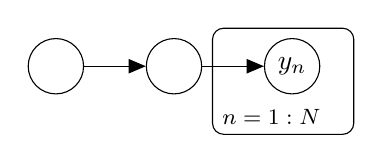
\begin{tikzpicture}
  \node[latent](theta) at (-3.0,0) {$\vtheta$};
  \node[latent](fn) at (-1.5,0) {$\vf$};
  \node[latent](yn) at (0,0) {$y_n$};
  \edge{theta}{fn};
  \edge{fn}{yn};
  \plate[xshift=0.3cm] {fy} {(yn)} {\hspace{0.3cm}$n=1:N$};
\end{tikzpicture}
\label{fig:gm-hierarchical}
\end{figure}
As an alternative, you could perform an always true product rule decomposition on $\vf$ as $p(\vf) = p(f_1)p(f_2|f_1)p(f_3|f_2,f_1)\dots$. This would result in a more complicated graphical model, which would also represent the dependence of $y_n$ on \emph{only} $f_n$.


\subsection{\questionref{q:gm-reflection}}
In the case of one object of colour $C$ under illumination $I$ reflecting light $L$ the meaningful factorisation of the joint distribution into tractable distributions was $p(C, L, I) = p(L|C, I) p(C, I) = p(L|C, I) P(C) p(I)$. Intuitively, given a colour and illumination, we could determine what the reflected light looks like ($p(L|C, I)$ term) and we assume that the illumination and `intrinsic' colour of the object are independent variables ($p(C, I) = p(C) p(I)$).

In the case with two objects, each will have its own intrinsic colour, which we denote as $C_1$ and $C_2$, and will reflect light differently with variables $L_1$ and $L_2$. Since we have on further information about the relationship of the items, it is safe to assume their intrinsic colours will be independent, so $p(C_1, C_2) = p(C_1) p(C_2)$. Similarly, there is no relationship between colour of the objects and illumination so $p(C_1, C_2, I) = p(C_1) p(C_2) p(I)$. Moreover, it is safe to assume that $L_1$ will depend on $C_1$ and $I$ only and $C_2$ will depend only on $C_2$ and $I$ and so $p(L_1, L_2|C_1, C_2, I)=p(L_1|  L_2, C_1, C_2, I) p(L_2| C_1, C_2, I)=p(L_1|  C_1, I) p(L_2| C_2, I)$. Hence, the joint will factorise as
\begin{align}
p(C_1, C_2,  L_1, L_2, I) &= p(L_1, L_2|C_1, C_2, I) p(C_1, C_2, I) \\
&= p(L_1, |C_1, I) p(L_2| C_2, I) p(C_1) p(C_2) p(I)
\end{align}
which is represented in the graphical model in Figure \ref{fig:gm-reflection}.
\begin{figure}[h]
\centering
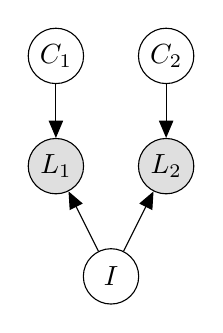
\begin{tikzpicture}
  \node[latent](c1) at (0,1.4) {$C_1$};
  \node[latent](c2) at (1.4,1.4) {$C_2$};
  \node[obs](l1) at (0,0) {$L_1$};
  \node[obs](l2) at (1.4, 0) {$L_2$};
  \node[latent](i) at (0.7, -1.4) {$I$};
  \edge{c1,i}{l1};
  \edge{c2,i}{l2};
%  \plate {xy} {(x)(y)} {$n=1,\dotsc, N$} ;
\end{tikzpicture}
\hspace{3.0cm}
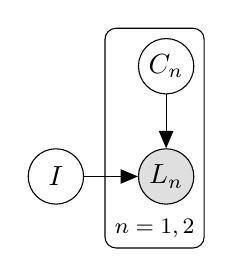
\begin{tikzpicture}
  \node[latent](i) at (0,0) {$I$};
  \node[latent](c) at (1.4,1.4) {$C_n$};
  \node[obs](l) at (1.4,0) {$L_n$};
  \edge{i}{l};
  \edge{c}{l};
  \plate {cl} {(c)(l)} {$n=1,2$} ;
\end{tikzpicture}
\caption{Graphical model representation of the reflection model. The graphical model on the right a compact but equivalent version of the one on the left.}
\label{fig:gm-reflection}
\end{figure}



\subsection{\questionref{q:gm-filtering}}
\subsubsection{Graphical Model Illustration}
\begin{figure}[h]
\centering
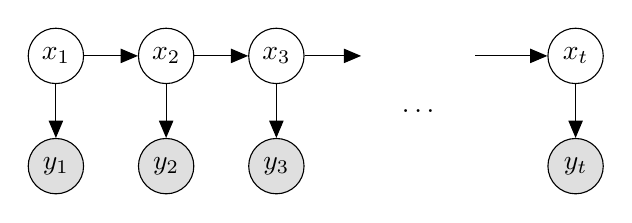
\begin{tikzpicture}
  \node[latent](x1) at (0,1.4) {$x_1$};
  \node[latent](x2) at (1.4,1.4) {$x_2$};
  \node[latent](x3) at (2.8,1.4) {$x_3$};
  \node[obs](y1) at (0,0) {$y_1$};
  \node[obs](y2) at (1.4,0) {$y_2$};
  \node[obs](y3) at (2.8,0) {$y_3$};
  \node(b1) at (4.0,1.4) {};
  \node(dots) at (4.6,0.7) {$\ldots$};
  \node(b2) at (5.2,1.4) {};
  \node[latent](xt) at (6.6,1.4) {$x_t$};
  \node[obs](yt) at (6.6,0) {$y_t$};
  \edge{x1}{y1};
  \edge{x2}{y2};
  \edge{x3}{y3};
  \edge{x2}{x3};
  \edge{x1}{x2};
  \edge{x3}{b1};
  \edge{b2}{xt};
  \edge{xt}{yt};
\end{tikzpicture}
\caption{Directed graphical model for the joint distribution given.}
\label{fig:gm-filtering}
\end{figure}

\subsubsection{Na\"{i}ve inference}
\label{sec:gm-filtering-naive}
Each $x_i$ may take one of $D_x$ values, and for brute force marginalisation as per $
p( x_t | \vy_{:t} ) = \sum_{x_1, \ldots, x_t} p( \vx_{:t}, \vy_{:t} ) / p( \vy_{:t} ) $, we would need to sum over \textit{all possible variable combinations}. Therefore, we would need sum over $(D_x)^t$ terms. Strictly speaking, if we neglect calculating $p( \vy_{:t} )$ explicitly, and instead reach the posterior by computing $p( x_{t}, \vy_{:t} )$ and then normalising over $x_t$ as $p( x_t | \vy_{:t} ) = p( x_{t}, \vy_{:t} ) / \sum_{x_t} p( x_{t}, \vy_{:t} )$, we would need to compute an additional sum over $x_t$. Total terms to sum over would therefore be $(D_x)^t + D_x$.

\subsubsection{Recursive inference}
If we know $p( x_{t-1} | \vy_{:t-1} )$, we can write the posterior at step $t$ as
\begin{align}
p(x_t | \vy_{:t}) &\stackrel{\text{AT}}{=} \sum_{x_{t-1}=1}^{D_x} \frac{ p( x_t, y_t, x_{t-1} | \vy_{:t-1} ) }{ p( y_t | \vy_{:t-1} ) } \\
&\stackrel{\text{MA}}{=} \sum_{x_{t-1}=1}^{D_x} \frac{ p( x_t | x_{t-1} ) p( y_t | x_t ) p( x_{t-1} | \vy_{:t-1} ) }{ p(y_t | \vy_{:t-1} ) }.
\end{align}
So to get from $p( x_{t-1} | \vy_{:t-1} )$ to the posterior at $t$, we need to sum over a single variable $x_{t-1}$, which can take one of $D_x$ values. Therefore, there are $D_x$ terms in the sum. As above, we would have to sum over an additional $D_x$ to normalise.

Also, notice that:
\begin{align}
p(x_{t+1}|y_{1:t}) &\stackrel{\text{AT}}{=} \sum_{x_t} p(x_{t+1},x_t|y_{1:t}) \\
&\stackrel{\text{AT}}{=} \sum_{x_t} p(x_{t+1}|x_t,y_{1:t}) p(x_t|y_{1:t}) \\
&\stackrel{\text{MA}}{=} \sum_{x_t} p(x_{t+1}|x_t) p(x_t|y_{1:t}) \,,
\end{align}
which is in the numerator of what was derived above.

\subsubsection{Comparison}
We are asked to evaluate how many terms we must sum over when we carry out sequential filtering to get $p( x_t | \vy_{:t} )$. In this case we need to sum over $x_{i-1}$ to calculate the update at each step for $1<i<t$, i.e. $t-1$ times. We also need to normalise over $x_t$ to get the final posterior. We thus calculate $t$ sums, each with $D_x$ terms, summing over a total of $D_x^t$ terms.

How does this compare with the brute force approach in \ref{sec:gm-filtering-naive}? Our answers show that using sequential filtering reduces the complexity from exponential to linear in $t$. This is a massive saving, particularly for large $t$. 



\subsection{\questionref{q:cp-binomial}}
\label{ans:cp-binomial}
We are asked to derive a conjugate prior $p( \theta )$ for a binomial likelihood $p( D | \theta ) = \theta^{ N_1 } \cdot( 1 - \theta )^{ N_0 }$. The posterior for a conjugate prior has the same form as the prior, but with different parameters, so we know that
\begin{align}
p( \theta | D ) &= \frac{ 1 }{ Z } p( \theta ) p( D | \theta )\\
&= \frac{1}{Z} p( \theta ) \theta^{ N_1 } \cdot( 1 - \theta )^{ N_0 }
\end{align}
shares the form of $p( \theta )$. $Z$ is a normalising constant which, as the question reminds us, we need not evaluate.

We can see that choosing a prior with similar form to the likelihood, we can simply collect the exponents of $\theta$ and $1 - \theta$ to get the corresponding parameters of the posterior. i.e.
\begin{align}
p( \theta ) = p( \theta ; a, b) &= \frac{ 1 }{ Z_\theta } \theta^{ a } \cdot( 1 - \theta )^{ b }\\
p( \theta | D ) &= \frac{ 1 }{ Z' } \theta^{ a + N_1 } \cdot( 1 - \theta )^{ b + N_0 } = p( \theta ; a + N_1, b + N_0 )
\end{align}
where $Z' = Z \cdot Z_\theta$ and $a, b$ are chosen prior parameters (or hyperparameters). Our conjugate prior is in fact a \textit{beta} distribution, which is more commonly written as
\begin{align}
p( \theta ; \alpha, \beta) &= \frac{ \theta ^ { \alpha - 1 } (1 - \theta ) ^ { \beta - 1} }{ \mathrm{ B }( \alpha, \beta )}.
\end{align}
$\mathrm{ B }( ., . )$ is known as the beta function. By comparing with the Bernoulli likelihood, we can see that $\alpha - 1$ and $\beta - 1$ act as pseudo-counts.

\subsection{\questionref{q:cp-exp-fam}}

\subsubsection{Show that the conjugate prior is given by $p(\eta|\tau, n_0) = H(\tau, n_0)\exp(\tau\transpose\eta - n_0 A(\eta))$: }
A prior is conjugate if the posterior is of the same family as the prior.
The given likeliood is 
\begin{align}
\ell(\eta) = p(x|\eta) = h(x) \exp\left(\eta\transpose t(x) - A(\eta)\right),
\end{align}
and the prior is
\begin{align}
p(\eta|\tau, n_0) = H(\tau, n_0)\exp(\tau\transpose\eta - n_0 A(\eta)).
\end{align}
We can find the posterior using
\begin{align}
p(\eta|x,\tau, n_0) &\propto p(\eta|\tau, n_0)p(x|\eta).
\end{align}
Computing this quantity is straightforward
\begin{align}
p(\eta|\tau, n_0)p(x|\eta) &= h(x)H(\tau, n_0) \exp\left(\eta\transpose t(x) - A(\eta) + \tau\transpose\eta - n_0 A(\eta) \right) \\
&= H'(x, \tau, n_0) \exp\left((t(x) + \tau)\transpose \eta - (1+n_0)A(\eta)\right), 
\end{align}
where $H'(x, \tau, n_0) = h(x)H(\tau, n_0)$.
As this is the same form as the prior, the prior is conjugate.

\subsubsection{Put the conjugate prior into the natural parameterisation.}

The natural parametrisation of the prior is as follows:
\begin{align}
p(\eta|\tau, n_0) = \exp \left(  \begin{bmatrix} \tau \\ n_0 \end{bmatrix}\transpose \begin{bmatrix} \eta \\ - A(\eta) \end{bmatrix}- (- \log H(\tau, n_0))  \right).
\end{align}
To write this in the natural parametrisation, we need to notice that $\tau, n_0$ are parameters of the prior and can be written with an inner product on functions of $\eta$.
The left over function of the parameters of the prior $H(\tau, n_0)$ can be taken inside the exponential, hence it can be written as the the log partition function. 


\subsection{\questionref{q:natural-form}}
The natural form for an exponential family distribution is
\begin{align}
p(x|\eta) = h(x) \exp\left(\eta\transpose t(x) - A(\eta)\right). \label{eq:natural-form}
\end{align}

\subsubsection{Gamma Distribution}
The pdf for a gamma distribution is
\begin{align}
p( x ; \alpha, \beta ) &= \frac{ x^ {\alpha - 1} \beta^\alpha \exp\left( - \beta x \right) }{ \Gamma(\alpha) }\\
&= \exp\left( ( \alpha - 1 ) \log x - \beta x - (\log \Gamma(\alpha) - \alpha \log \beta ) \right)
\end{align}
Comparing to \eqref{eq:natural-form} we see that
\begin{align}
h(x) &= 1 \\
\eta(\alpha, \beta) &= \begin{bmatrix} \alpha - 1 \\ -\beta \end{bmatrix} = \begin{bmatrix} \eta_1 \\ \eta_2 \end{bmatrix} \\
t(x) &=  \begin{bmatrix} \log x \\ x \end{bmatrix} \\
A(\eta) &= \log \Gamma (\eta_1 + 1) - ( \eta_1 + 1 ) \log(-\eta_2).
\end{align}
Equivalently, we could have chosen $\eta_1=\alpha$, $A(\eta)=\log \Gamma (\eta_1) - \eta_1 \log(-\eta_2)$ and $h(x) = 1 / x $.


\subsubsection{Beta Distribution}
Rearranging the pdf for a beta distribution, we have
\begin{align}
p( x ; \alpha, \beta ) &= \frac{ x^{ \alpha - 1} ( 1 - x )^{ \beta - 1 } }{ B( \alpha, \beta )} \\
&= \exp \left( ( \alpha - 1 ) \log x + ( \beta - 1 ) \log ( 1 - x ) - \log B( \alpha, \beta ) \right)\\
&= \exp \left( - \log x - \log ( 1 - x ) \right) \exp \left( \alpha \log x + \beta \log ( 1 - x ) - \log B( \alpha, \beta ) \right)\\
&= \frac{ 1 }{ x ( 1 - x ) } \exp \left( \alpha \log x + \beta \log ( 1 - x ) - \log B( \alpha, \beta ) \right).
\end{align}
Comparing to \eqref{eq:natural-form} we see that
\begin{align}
h(x) &= \frac{ 1 }{ x ( 1 - x ) } \\
\eta(\alpha, \beta) &= \begin{bmatrix} \alpha \\ \beta \end{bmatrix} = \begin{bmatrix} \eta_1 \\ \eta_2 \end{bmatrix} \\
t(x) &=  \begin{bmatrix} \log x \\ \log( 1 - x ) \end{bmatrix} \\
A(\eta) &= \log B (\eta_1, \eta_2 ).
\end{align}


\subsubsection{Univariate Gaussian Distribution}
The pdf for a univariate Gaussian distribution is
\begin{align}
p( x ; \mu, \sigma ) &= \frac{ 1 }{ \sqrt{2 \pi } \sigma } \exp\left( - \frac{ 1 }{ 2 } \frac{ (x - \mu )^2 }{ \sigma^2 } \right).\\
\intertext{Putting this into natural form, we have}
p( x ; \mu, \sigma ) &= \frac{ 1 }{ \sqrt{2 \pi} } \exp\left( -\log\sigma - \frac{ 1 }{ 2 \sigma ^2 } \left( x^2 - 2 x\mu + \mu^2 \right) \right)\\
&= \frac{ 1 }{ \sqrt{2 \pi} } \exp\left( - \left( \frac{ \mu^2 }{ 2 \sigma ^2 } + \log\sigma \right) - \frac{ 1 }{ 2 \sigma ^2 } x^2 + \frac{ \mu }{ \sigma ^2 } x  \right).
\end{align}
Comparing to \eqref{eq:natural-form} we see that
\begin{align}
h(x) &= h = \frac{ 1 }{ \sqrt{ 2 \pi } } \\
\eta(\mu, \sigma) &= \begin{bmatrix} \frac{ \mu }{ \sigma^2 } \\ -\frac{ 1 }{ 2 \sigma^2 } \end{bmatrix} = \begin{bmatrix} \eta_1 \\ \eta_2 \end{bmatrix} \\
t(x) &=  \begin{bmatrix} x \\ x^2 \end{bmatrix} \\
A(\eta) &= -\left( \frac{ \eta_1^2 }{ 4\eta_2 } + \frac{ 1 }{ 2 } \log(- 2\eta_2) \right).
\end{align}


\subsection{\questionref{q:cp-exp-fam-examples}}
\subsubsection{Bernoulli Likelihood}
The likelihood of the probability of success $\theta$ for a Bernoulli-distributed random variable is given by
\begin{align}
p( x | \theta) &= \theta^x ( 1 - \theta )^{( 1 - x )}.
\end{align}
Putting this into the exponential family form given in the question
\begin{align}
p( x | \theta) &= \exp  \log \left( \theta^x ( 1 - \theta )^{( 1 - x )} \right) \\
&= \exp  \left( x\log \frac{ \theta }{ 1 - \theta } + \log ( 1 - \theta ) \right)
\end{align}
we see that
\begin{align}
h(x) &= 1 \\
\eta &= \log \frac{ \theta }{ 1 - \theta } \\
t(x) &= x \\
A( \eta ) &= -\log \left( 1 - \frac{ e^\eta }{ 1 + e^\eta } \right) = \log ( 1 + e^\eta ).
\end{align}
Starting from the general exponential family conjugate prior we have shown in the previous question, we can find the Bernoulli conjugate prior
\begin{align}
p(\eta | \tau, n_0) &= H( \tau, n_0 ) \exp\left( \tau\transpose \eta - n_0 A(\eta) \right) \\
p(\theta | \tau, n_0)  &= H( \tau, n_0 ) \exp\left( \tau\transpose \log \frac{ \theta }{ 1 - \theta } + n_0 \log ( 1 - \theta ) \right) \\
&= H( \tau, n_0 ) \theta ^ \tau ( 1 - \theta ) ^ {n_0 - \tau}.
\end{align}
As discussed in Section~\ref{ans:cp-binomial}, this is a beta distribution, with parameters $\alpha=\tau + 1$ and $\beta=n_0-\tau + 1$. Its normalising constant is defined by the beta function: $H( \tau, n_0 )=1/B(\alpha,\beta)$.

\subsubsection{Gaussian likelihood with unknown precision but known mean}
The Gaussian likelihood, for a precision $\nu=1/\sigma^2$ is
\begin{align}
p(x|\mu,\nu) &= \sqrt{\frac{ \nu }{ 2\pi }} \exp\left(- \frac{ \nu }{ 2 } \left( x - \mu \right)^2 \right) \\
&= \sqrt{\frac{ \nu }{ 2\pi }} \exp\left(- \frac{ \nu }{ 2 } \left( x^2 - 2 x\mu + \mu^2 \right) \right). 
\end{align}
The parameters of the exponential family form are
\begin{align}
h(x) &= (2\pi)^{-\frac{1}{2}} \\
\eta &= \nu\\
t(x) &= -\frac{ 1 }{ 2 }\left( x^2 - 2x\mu \right)\\
A( \eta ) &=\frac{1}{2}\left( \nu\mu^2 - \log\nu\right).
\end{align}
Note that we have used the fact that $\mu$ is known and therefore does not appear in our natural parameters. Starting from the general exponential family conjugate prior, we can write
\begin{align}
p(\eta | \tau, n_0) &= H( \tau, n_0 ) \exp\left( \tau\transpose \eta - n_0 A(\eta) \right) \\
p(\nu | \mu, \tau, n_0)  &= H( \tau, n_0 ) \exp\left( \tau\nu - n_0 \frac{1}{2}\left( \nu\mu^2 - \log\nu\right) \right) \\
p(\nu | \mu, \tau, n_0)  &= H( \tau, n_0 ) \exp\left(\nu \left( \tau -  \frac{n_0 \mu^2}{2} \right)\right) \nu^{ \frac{ n_0 }{ 2 } }. 
\end{align}
This is in fact an \emph{inverse gamma} distribution on $\sigma^2$. Inverse gamma distributions are usually written in the form
\begin{align}
p(x | \alpha,\beta)=\frac{\beta^\alpha}{\Gamma(\alpha)}\left(\frac{1}{x}\right)^{\alpha + 1} \exp \left(-\beta / x \right)
\end{align}
where $\Gamma(\alpha)$ is known as the gamma function.



\subsection{\questionref{q:cp-gaussian}}
This question addresses multivariate Gaussian distributions: we will be setting all distributions in their natural form so we first tackle how to put in exponential family form the general multivariate Gaussian with mean $\vmu$ and covariance matrix $\Sigma$. For an $N$ dimensional distribution with likelihood model $p(x; \vmu, \Sigma)$, we start by rewriting
\begin{align}
\NormDist{\vx; \vmu, \Sigma} &= \frac{1}{(2 \pi \detbar{\Sigma})^\frac{N}{2}} \exp{-\left(\frac{1}{2}(\vx - \vmu)\transpose \Sigma^{-1} (\vx - \vmu)\right)}  \\
 & = \frac{1}{(2 \pi)^\frac{N}{2}} \exp{\left(-\frac{1}{2}\vx\transpose \Sigma^{-1} \vx + \vx\transpose \Sigma^{-1} \vmu -\frac{1}{2}\vmu\transpose\Sigma^{-1}\vmu - \frac{N}{2}\log\detbar{\Sigma}\right)}.
\end{align}
To write this in the required exponential form, we have to rearrange the term in the exponential so that somehow we have a `sufficient statistic' $t(x)$ term that is a function of the data dotted with vector $\eta$ that is some function of the parameters $\vmu, \Sigma$. This is straightforward for the term $\vx \transpose \Sigma^{-1} \vmu$, and for the term quadratic in $\vx$ we can use the following trick. We have
\begin{align}
\vx\transpose \Sigma^{-1} \vx &= \sum_{i,j} x_i \Sigma^{-1}_{i, j} x_j \\
&= \sum_{i,j} x_i \Sigma^{-1}_{i, j} x_j \\
& = \sum_{i, j} \Sigma^{-1}_{i,j} x_i x_j \\
& = \overrightarrow{\left(\vx \vx\transpose\right)} \overrightarrow{\left(\Sigma^{-1}\right)},
\end{align}
where $\vx \vx\transpose$ is a matrix with element $i,j$ equal to $x_i x_j$ and the notation $\overrightarrow{\left(\cdot\right)}$ denotes that we are flattening the relevant matrix into a vector (preserving the ordering so that all matrices are flattened in the same way). We have now written the quadratic term in the required form of a dot product (between two $N^2$ dimensional vectors) where one is a function of $\vx$ and the other is in terms of the distribution parameters $\vmu, \Sigma$.

Substituting into our previous expression gives
\begin{align}
\NormDist{\vx; \vmu, \Sigma} &= \frac{1}{(2 \pi)^\frac{N}{2}} \exp{\left(-\frac{1}{2} \overrightarrow {\vx \vx\transpose} \overrightarrow{\Sigma^{-1}} + \vx\transpose \Sigma^{-1} \vmu -\frac{1}{2}\vmu\transpose\Sigma^{-1}\vmu - \frac{N}{2}\log\detbar{\Sigma}\right)} \\
& =  \frac{1}{(2 \pi)^\frac{N}{2}} \exp{\left(\begin{bmatrix} \vx \\ \overrightarrow{\vx\vx\transpose}\end{bmatrix}\transpose \begin{bmatrix}\Sigma^{-1}\mu \\ -\overrightarrow{\Sigma^{-1}}/2\end{bmatrix} -\left(\frac{1}{2}\vmu\transpose\Sigma^{-1}\vmu + \frac{N}{2}\log\detbar{\Sigma}\right)\right)}
\end{align}
and comparing with the standard form of the exponential family $p(\vx|\eta) = h(x) \exp(\eta\transpose t(x) - A(\eta))$, we can now make the immediate identifications $h(x) = \left(2\pi\right)^{-\frac{N}{2}}$, $t(x) = \begin{bmatrix} \vx & \overrightarrow{\vx\vx\transpose}\end{bmatrix}\transpose$ and $\eta = \begin{bmatrix} \Sigma^{-1}\vmu & -\overrightarrow{\Sigma^{-1}}/2\end{bmatrix}\transpose$. Finally, we identify $A(\eta) = \frac{1}{2}\vmu\transpose\Sigma^{-1}\vmu + \frac{N}{2}\log\detbar{\Sigma}$, which we could in principle rewrite as a function of the elements of $\eta$ to determine $A(\eta)$ explicitly. For this question this implicit form of $A(\eta)$ will suffice.

Applying our general formula to the particular multivariate Gaussians of interest to the question we recover for the likelihood
\begin{equation}
p(\vy| \vf) = \NormDist{\vy; \vf, \sigma^2 \mathrm I_N} =  \frac{1}{\left( {2\pi}\right)^\frac{N}{2} } \exp{\left(\begin{bmatrix} \vy  \\ \overrightarrow{\vy\vy\transpose}\end{bmatrix}\transpose\begin{bmatrix} \vf/\sigma^2 \\ -\mathrm I_N/(2\sigma^2)\end{bmatrix} - \frac{1}{2\sigma^2} \vf\transpose\vf - \frac{N}{2} \log{\sigma^2} \right)}
\end{equation}
with $h_l(y) = \left(2\pi\right)^{-\frac{N}{2}}$,  $\eta_l = \begin{bmatrix} \vf/\sigma^2 & -\mathrm I_N/(2\sigma^2)\end{bmatrix}\transpose$, $t_l(y) = \begin{bmatrix} \vy & \overrightarrow{\vy\vy\transpose}\end{bmatrix}\transpose$ and implicit $A_l(\eta_l) = \frac{1}{2\sigma^2} \vf\transpose\vf -\frac{N}{2} \log{\sigma^2}$.

Note that in this case the likelihood above could also be simplified as 
\begin{align}
p(\vy| \vf) &=  \frac{1}{\left( {2\pi}\right)^\frac{N}{2} } \exp{\left(-\frac{1}{2\sigma^2}\vy\transpose\vy+\frac{1}{\sigma^2}\vy\transpose\vf-\frac{1}{2\sigma^2}\vf\transpose\vf - \frac{N}{2} \log{\sigma^2}\right) } \\
&=  \frac{1}{\left( {2\pi}\right)^\frac{N}{2} } \exp{\left(\begin{bmatrix} \vy  \\ \vy\transpose\vy\end{bmatrix}\transpose\begin{bmatrix} \vf/\sigma^2 \\ -1/(2\sigma^2)\end{bmatrix} - \frac{1}{2\sigma^2} \vf\transpose\vf - \frac{N}{2} \log{\sigma^2} \right)}
\end{align}
which would result in an alternative but equivalent parametrisation in exponential family form with lower dimensional $\eta$ and $t(y)$ vectors.

Moving on to the prior, we recover
\begin{equation}
\NormDist{\vf; 0, \mathrm K} =  \frac{1}{ (2 \pi)^\frac{N}{2}}  \exp{\left(\begin{bmatrix} \vf \\ \overrightarrow{\vf  \vf \transpose}\end{bmatrix}\transpose\begin{bmatrix} \vec{0} \\ -\frac{1}{2}\overrightarrow{\mathrm K^{-1}}\end{bmatrix} - \frac{N}{2} \log{\detbar{\mathrm K}}\right)}
\end{equation}
with corresponding parametrisation $h_p(f) = (2\pi)^{-\frac{N}{2}}$, $\eta_p =  \begin{bmatrix}\vec{0} & -\frac{1}{2}\overrightarrow{\mathrm K^{-1}}\end{bmatrix}$, $t_p(f) = \begin{bmatrix} \vf & \overrightarrow{\vf  \vf \transpose}\end{bmatrix}\transpose$ and $A_p(\eta_p) = \frac{N}{2} \log\detbar{\mathrm K}$.

Now, to ascertain that the two distributions are conjugate, we look at the form of the posterior. By multiplying the two, we see it will be proportional to
\begin{align}
p(f|y) &\propto \exp{\left(\begin{bmatrix} \vy  \\ \overrightarrow{\vy\vy\transpose}\end{bmatrix}\transpose\begin{bmatrix} \vf/\sigma^2 \\ -\mathrm I_N/(2\sigma^2)\end{bmatrix} - \frac{1}{2\sigma^2} \vf\transpose\vf - \frac{N}{2} \log{\sigma^2} + \begin{bmatrix} \vf \\ \overrightarrow{\vf  \vf \transpose}\end{bmatrix}\transpose\begin{bmatrix} \vec{0} \\ -\frac{1}{2}\overrightarrow{\mathrm K^{-1}}\end{bmatrix} - \frac{N}{2} \log{\detbar{\mathrm K}}\right)} \\
&\propto  \exp{\left(
\underbrace{\begin{bmatrix}\vf \\ \overrightarrow{\vf  \vf \transpose}\end{bmatrix}\transpose}_{t(f)}
\underbrace{\begin{bmatrix} \vy/\sigma^2 \\ -\frac{1}{2}\left(\overrightarrow{\mathrm K^{-1}}+\overrightarrow{\mathrm I_N} / \sigma^2\right)\end{bmatrix}}_{\eta}
-\underbrace{\left(\vy\transpose\mathrm K^{-1}\vy+ \frac{N}{2} (\log{\sigma^2} + \log{\detbar{\mathrm K}})\right)}_{A(\eta)}
\right)}
\end{align}
and we have the posterior in exponential family form (so the two distributions are conjugate), with the normalisation constant $h$ that could be found by normalising the expression with respect to $\vf$.





\subsection{\questionref{q:lmgp-cert}}
We assume the following model
\begin{align}
p(\vtheta) &= \mathcal{N}(\mathbf{0}, \mathbf{I}_M), \\
p(\vy| \mathbf{X}, \vtheta) &= \mathcal{N}(\mathbf{\Phi}(\mathbf{X}) \vtheta, \sigma^2\mathbf{I}_N), 
\end{align}
where $\mathbf{\Phi}(\mathbf{X})$ is a $N \times M$ matrix and $M$ is the number of basis functions.
The posterior on $\vtheta$ will be Gaussian as 
\begin{align}
p(\vtheta| \vy, \mathbf{X}) \propto p(\vy| \vtheta, \mathbf{X})p(\vtheta),
\end{align}
and both the likelihood and prior are Gaussian, and the likelihood is a linear function of the parameter.
Looking at just the variance (you should be able to derive this on your own), we get 
\begin{align}
\Sigma_{\vtheta|\vy, \mathbf{X}} = \mathbf{I}_M - \mathbf{\Phi}(\mathbf{X}) \transpose \left[  \mathbf{\Phi}(\mathbf{X})\mathbf{\Phi}(\mathbf{X}) \transpose + \sigma^2 \mathbf{I}_N\right]^{-1} \mathbf{\Phi}(\mathbf{X}).
\end{align}
If we have $M$ distinct datapoints, $\mathbf{\Phi}(\mathbf{X})$ is an $M \times M$ matrix and is full rank and hence invertible.
We take $\sigma^2 \rightarrow 0$ as that is the likelihood noise.
Then,
\begin{align}
\Sigma_{\vtheta|\vy, \mathbf{X}} &= \mathbf{I}_M - \mathbf{\Phi}(\mathbf{X}) \transpose   (\mathbf{\Phi}(\mathbf{X}) \transpose) ^{-1}\mathbf{\Phi}(\mathbf{X}) ^{-1}  \mathbf{\Phi}(\mathbf{X}). \\
 &= \mathbf{0}
\end{align}

\subsection{\questionref{q:gp-rv}}
For an alternative explanation, see \citet[p.~13]{gpml}.

A scalar function $f: \Reals^D\to \Reals$ can be seen as a collection of scalar output variables indexed by some input $\vx \in \Reals^D$. In this case where inputs lie in the vector space $\Reals^D$, the number of variables in the collection is infinite\footnote{Or more specifically, \emph{uncountably} infinite, but for the purpose of this course this is a detail of minor importance.}, since there are an infinite number of inputs.\footnote{In the course, we will consider only inputs in $\Reals^D$. However you can have functions on many different types of inputs, leading to different sizes of the set of output variables. For example, you could have a function from a finite set: $\{0, 1, 2, 3, 4\} \to \Reals$.} We can consider finite subsets of the output variables that correspond to finite subsets of inputs. I.e.~for a set of $N$ inputs
\begin{align}
X = \{\vx_1, \dots, \vx_N\} \,,
\end{align}
which we can also denote as a matrix $X \in \Reals^{N\times D}$, we have the corresponding output set
\begin{align}
f(X) = \{f(\vx_1), \dots, f(\vx_N)\} \,,
\end{align}
which we alternatively denote as a vector $f(X) \in \Reals^N$. If the entire function $f(\cdot)$ is a random variable with some distribution, this will also mean that the function outputs $f(X)$ will be a random variable with some distribution.

Going back to the abstract definition of a Gaussian process, we see that its definition as a collection of random variables matches what we found must hold for a function-valued random variable. The collection of random variables that form the Gaussian process can be identified with the random variables of the function outputs at specified inputs. The next part of the definition specifies that a finite subset of the random variables in the Gaussian process must be Gaussian distributed, i.e.~for some arbitrary set of inputs $X$, the corresponding set of outputs $f(X)$ is Gaussian distributed
\begin{align}
f(\cdot) \sim \mathcal{GP} \implies p(f(X)) = \NormDist{f(X); \vmu_{f(X)}, \boldsymbol{\Sigma}_{f(X)}} \,,
\end{align}
with some mean $\vmu_{f(X)} \in \Reals^N$ and covariance matrix $\boldsymbol{\Sigma}_{f(X)} \in \Reals^{N\times N}$. The value of $X$ determines \emph{which} random variables in the collection of the GP we are considering, and therefore must also determine the value of $\vmu_{f(X)}$ and $\boldsymbol{\Sigma}_{f(X)}$.

\textbf{So, long story short:} When we use a Gaussian process as a distribution over functions, the random variables in the collection that makes up the GP are used as the \emph{outputs of the function at some input locations}.


\subsection{\questionref{q:mean-cov-determine-gp}}
True.

\subsection{\questionref{q:prior-density}}
The mean function $\mu: \Reals^D \to \Reals$ and covariance function\footnote{The covariance function is often referred to as the \emph{kernel}.} $k: \Reals^D \times \Reals^D \to \Reals$ determine the mean vector and covariance matrix of the distribution over function values for some input. For example, for the inputs $X$, we have
\begin{gather}
p(f(X)) = \NormDist{f(X); \vmu_{f(X)}, \boldsymbol{\Sigma}_{f(X)}} \,, \\
\text{with } \left[\vmu_{f(X)}\right]_n = \mu(\vx_n)\,, \quad \text{and } \left[\boldsymbol{\Sigma}_{f(X)}\right]_{nn'} = k(\vx_n, \vx_{n'}) \,,
\end{gather}
where $[\dots]_{n}$ denotes indexing a vector or matrix. We will often denote the covariance matrix of a common set of inputs (e.g.~training inputs $X$) as $\K$. Alternatively, we can denote the matrix resulting from evaluating the covariance function at two sets of inputs $X \in \Reals^{N\times D}, X^*\in \Reals^{N^*\times D}$ as
\begin{align}
K(X, X^*) \in \Reals^{N\times N^*} \,.
\end{align}

\subsection{\questionref{q:posterior}}
In inference problems, the goal is to go from a joint probability distribution over all relevant variables (which comes from the model specification) to a conditional distribution given observations (the posterior). The posterior is obtained by manipulating the joint using the rules of probability. Often Bayes' rule is enough, but sometimes other applications of the product or sum rules are necessary \citep[p.~24]{itila}. I will go through this derivation multiple ways, and in quite a lot of detail. I will pay special attention to the manipulations of the probability distributions on the way, as it is important to be familiar with how to do this. If you struggle with this, I would recommend looking over chapters 1--3 of \citet{itila}, and perhaps doing a few exercises.

\subsubsection{Understanding and manipulating the joint}
The joint distribution is usually specified through a set of conditional probability distributions. For Gaussian process regression, the problem specification gives:
\begin{enumerate}
\item The \emph{prior} distribution over the function values at any inputs, through the definition of the prior over functions being a GP. For a set of inputs $X$, we can refer to the prior density over corresponding function values as $p(f(X))$.
\item The conditional distribution of any observation $y_n$ at an input location $\vx_n$, conditioned on full knowledge of the underlying function value. This distribution is known as the \emph{likelihood}, and is written as $p(y_n\given f(\vx_n), \vx_n)$ in this case, and has the density $\NormDist{y_n; f(\vx_n), \sigma^2}$.
\end{enumerate}
We need to consider the function values at both the training points $f(X)$ and testing points $f(X^*)$, in addition to the outputs $\vy$. This gives us the joint distribution $p(f(X), f(X^*), \vy\given X)$.
We can factorise the joint along the conditional independence relationships that the model was specified with:
\begin{align}
p(f(X), f(X^*), \vy\given X) &= p(f(X), f(X^*))p(\vy\given f(X), X) \\
&= p(f(X), f(X^*)) \prod_{n=1}^N p(y_n\given f(\vx_n), \vx_n) \,.
\end{align}
We can also go one step further and factorise the prior using \cref{eq:gauss-cond-joint,eq:gauss-cond}:
\newcommand{\Kff}{\K_{\vf\vf}}
\newcommand{\Kfp}{\K_{\vf\vf^*}}
\newcommand{\Kpp}{\K_{\vf^*\vf^*}}
\begin{align}
p(f(X), f(X^*)) &= \NormDist{\begin{bmatrix}f(X) \\ f(X^*)\end{bmatrix}; 0, \begin{bmatrix}\Kff & \K_{\vf\vf^*} \\ \K_{\vf\vf^*}\transpose & \K_{\vf^*\vf^*}\end{bmatrix}} \\ % = \NormDist{\begin{bmatrix}f(X) \\ f(X^*)\end{bmatrix}; 0, \begin{bmatrix}k(X, X) & k(X, X^*) \\ k(X^*, X) & k(X^*, X^*)\end{bmatrix}} \\
\implies p(f(X^*)\given f(X)) &= \NormDist{f(X^*); \Kfp\transpose\Kff\inv f(X), \quad \Kpp  - \Kfp\transpose\Kff\inv\Kfp} \label{eq:gp-prior-factorisation} \,,
\end{align}
where $\Kff = k(X, X)$, $\Kfp = k(X, X^*)$, and $\Kpp = k(X^*, X^*)$.
This gives an overall factorised joint of
\begin{align}
p(f(X), f(X^*), \vy\given X) &= p(f(X)) p(f(X^*)\given p(f(X))) \prod_{n=1}^N p(y_n\given f(\vx_n), \vx_n)
\end{align}
This conditional independence relationship can be represented as a graphical model, which often helps in reasoning about the model (\cref{fig:gp-gm})

\begin{figure}[h]
\centering
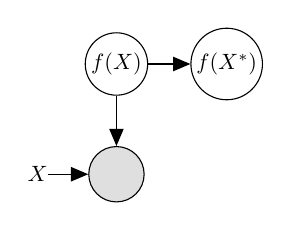
\begin{tikzpicture}
  \node[latent](fx) at (0,1.4) {\fixgmfont{$f(X)$}};
  \node[latent](fxp) at (1.4,1.4) {\fixgmfont{$f(X^*)$}};
  \node[obs](y) at (0,0) {$\vy$};
  \node[const](x) at (-1,0) {\fixgmfont{$X$}};
  \edge{fx,x}{y};
  \edge{fx}{fxp};
%  \plate {xy} {(x)(y)} {$n=1,\dotsc, N$} ;
\end{tikzpicture}
\hspace{3.0cm}
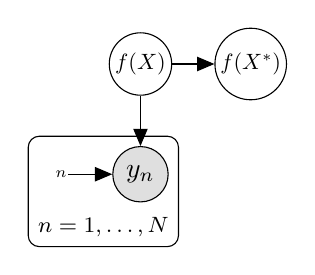
\begin{tikzpicture}
  \node[latent](fx) at (0,1.4) {\fixgmfont{$f(X)$}};
  \node[latent](fxp) at (1.4,1.4) {\fixgmfont{$f(X^*)$}};
  \node[obs](y) at (0,0) {$y_n$};
  \node[const](x) at (-1,0) {\fixgmfont{$\vx_n$}};
  \edge{fx,x}{y};
  \edge{fx}{fxp};
  \plate {xy} {(x)(y)} {$n=1,\dotsc, N$} ;
\end{tikzpicture}
\caption{Graphical model representations of Gaussian process regression, with conditional independence of $\vy$ represented explicitly on the right.}
\label{fig:gp-gm}
\end{figure}




We are tasked with finding the posterior over function values at an arbitrary set of input locations $X^*$, given that we observe a training set consisting of $N$ inputs and corresponding outputs $\{\vx_n, y_n\}_{n=1}^N$. We arrange the inputs into a matrix $X \in \Reals^{N\times D}$, and the outputs into a vector $\vy\in\Reals^N$.

\subsubsection{Method 1: Starting with the appropriate joint}
\label{sec:joint}
One representation of Bayes' rule that we can apply is the joint distribution divided by the conditional. In our case this becomes
\begin{align}
p(f(X^*)\given \vy, X) = \frac{p(\vy, f(X^*)\given X)}{p(\vy\given X)} \,.
\end{align}
However, the model specification did not give us the density of $p(\vy, f(X^*)\given X)$, so we will have to find it ourselves. We can find it by marginalising (or \emph{integrating out}) the unused variable $f(X)$ from the joint using the sum rule:
\begin{align}
p(\vy, f(X^*)) = \int p(\vy, f(X), f(X^*)\given X) \calcd{f(X)} \,.
\end{align}
We know the joint is a Gaussian, as the conditionals are all Gaussians which only interact linearly. This makes the marginal Gaussian too. We could perform the integration by hand, but given the knowledge that $p(\vy, f(X^*)\given X)$ is Gaussian, we could also just compute its means and covariances. The means are all zero. The main useful insight into finding the covariances, is that the Gaussian likelihood can be rewritten as
\begin{align}
\vy = f(X) + \boldsymbol{\epsilon}\,, \qquad \boldsymbol{\epsilon} \sim \NormDist{0, \sigma^2\mathbf{I}_N} \,.
\end{align}
This makes the covariances
\begin{align}
\Cov\left[\vy, f(X^*)\right] &= \Exp{f, \vepsilon}{\left(f(X) + \vepsilon\right)f(X^*)\transpose} = \Exp{f, \vepsilon}{f(X)f(X^*)\transpose} + \cancelto{0}{\Exp{f,\vepsilon}{\vepsilon f(X^*)\transpose}} \\
&= k(X, X^*) = \Kfp \,, \\
\Cov[\vy, \vy] &= \Exp{f, \vepsilon}{\left(f(X) + \vepsilon\right)\left(f(X)+\vepsilon\right)\transpose} = k(X, X) + \sigma^2\mathbf{I} = \Kff + \sigma^2\mathbf{I} \,, \\
\Cov[f(X^*), f(X^*)] &= k(X^*, X^*) = \Kpp \,.
\end{align}

The posterior can now be found by simple Gaussian conditioning, using \cref{eq:gauss-cond-joint,eq:gauss-cond}:
\begin{align}
p(\vy, f(X^*)\given X) &= \NormDist{\begin{bmatrix}\vy \\ f(X^*)\end{bmatrix}; 0, \begin{bmatrix}\Kff + \sigma^2\mathbf{I}_N & \K_{\vf\vf^*} \\ \K_{\vf\vf^*}\transpose & \K_{\vf^*\vf^*}\end{bmatrix}} \\ % = \NormDist{\begin{bmatrix}f(X) \\ f(X^*)\end{bmatrix}; 0, \begin{bmatrix}k(X, X) & k(X, X^*) \\ k(X^*, X) & k(X^*, X^*)\end{bmatrix}} \\
\implies p(f(X^*)\given \vy, X) &= \NormDist{f(X^*); \Kfp\transpose(\Kff+\sigma^2\mathbf{I})\inv \vy, \quad \Kpp  - \Kfp\transpose(\Kff+\sigma^2\mathbf{I})\inv\Kfp} \,.
\end{align}
This completes the exercise.

\subsubsection{Method 2: Finding a larger posterior then marginalising}
\label{sec:larger-posterior}
Alternatively, we may want to apply Bayes' rule directly. However, our joint also contains $f(X)$, which we weren't interested in representing in our posterior. We can also solve the problem by applying Bayes' rule to find the posterior $p(f(X), f(X^*)\given\vy, X)$, and then marginalising out $f(X)$. We start by applying Bayes' rule to the usual prior-likelihood factorisation of the joint:
\begin{align}
p(f(X), f(X^*)\given \vy, X) = \frac{p(\vy\given f(X), X) p(f(X), f(X^*))}{p(\vy\given X)} \,.
\end{align}
The first thing we can notice is that using the factorisation of the prior from \cref{eq:gp-prior-factorisation}, we can actually write the posterior over both training and testing points in terms of the posterior over only the training points:
\begin{align}
p(f(X), f(X^*)\given \vy, X) &= \frac{p(\vy\given f(X), X) p(f(X))}{p(\vy\given X)} p(f(X^*)\given f(X)) \\
&= p(f(X)\given \vy) p(f(X^*)\given f(X))
\end{align}
We then marginalise out $f(X)$ to get the posterior we are interested in:
\begin{align}
p(f(X^*)\given\vy) = \int p(f(X)\given \vy) p(f(X^*)\given f(X))\calcd{f(X)} \,.
\end{align}

Performing these computations requires exactly the same procedure of forming the joint and performing Gaussian conditioning (\cref{eq:gauss-cond-joint,eq:gauss-cond}) as in the previous way. 
Once the joint $p(f(X), f(X^*)\given \vy)$ is obtained, marginalisation can be performed simply by dropping the rows and columns related to $f(X)$ from the covariance. Overall the process is a bit more laborious than the other method.\footnote{However, it does give us the nice insight that the only part of the posterior that \emph{really} changes due to the data is $p(f(X)\given\vy)$, and that any change in the posterior on $f(X^*)$ only occurs \emph{through} the effect on $f(X)$.}



\subsection{\questionref{q:marginalisation}}
The Gaussian process prior defines a joint distribution over all finite subsets of the infinite set of function values. This raises the question of \emph{which} finite subset we need to represent in order to do inference. We know that we at least need to represent $f(X)$ for the training data $X$, since these function values are involved in the likelihood. If we want to make predictions over some new subset of input points $X^*$, these need to be involved in inference as well. The question remains, do we need to represent any other points?

We only need to represent variables that influence the inference over variables we are interested in. To consider whether we need to represent any other function values, we can include them in our posterior analysis, integrate them out, and see whether they influence our beliefs in what we are interested in. We can do this by repeating the derivation in \cref{sec:larger-posterior}, but with extra function values $f(\tilde{X})$ included.
\begin{align}
p(f(X), f(X^*), f(\tilde{X})\given \vy, X) &= \frac{p(\vy\given f(X), X) p(f(X))}{p(\vy\given X)} p(f(X^*)\given f(X)) p(f(\tilde X)\given f(X), f(X^*)) \\
&= p(f(X)\given \vy) p(f(X^*)\given f(X)) p(f(\tilde X)\given f(X), f(X^*))
\end{align}
By integrating out $f(\tilde X)$ we see that the posterior given by this procedure is the same as the posterior which we obtained without considering the extra points $f(\tilde X)$. Because this holds for \emph{any} set of other points $\tilde X$, this shows that including any other set of points doesn't change the outcome of our inference procedure, and therefore we don't have to include them in the first place.

If you look at the derivation, you actually see that the fact that the prior over function values defines consistent distributions over function values. The distributions are consistent in the sense that if we consider the prior joint $p(f(X), f(X^*))$ and integrate out $f(X^*)$, then we get the same distribution as if we had considered the prior $p(f(X))$ directly. This is a direct consequence of a Gaussian process being a distribution over functions.

It is, of course, possible to define an infinite collection of probability densities that do not have this property. For example, defining the precision of a Gaussian using a covariance function. See \citet[\S 2.2]{gpml} for another explanation.




\subsection{\questionref{q:pred-obs}}
An observation $y_n$ is modelled by the function value $f(\vx_n)$ with some noise added. This question is asking for a posterior distribution over a different random variable than \cref{q:posterior} (i.e.~$y_n$, rather than $f(\vx_n)$). Once you have the posterior of $f(\vx_n)$, you can use the usual manipulations of Gaussian distributions to find out that you just need to add $\sigma^2 \mathbf{I}_{N^*}$ to the covariance, where $N^*$ is the number of test points. You could also apply Bayes' rule to the joint distribution
\begin{align}
p(\vy^*\given \vy, X, X^*) &= \frac{p(\vy, \vy^*\given X, X^*)}{p(\vy\given X)} \\
&= \NormDist{\begin{bmatrix}\vy \\ \vy^*\end{bmatrix}; 0, \begin{bmatrix}\Kff + \sigma^2\mathbf{I}_N & \K_{\vf\vf^*} \\ \K_{\vf\vf^*}\transpose & \K_{\vf^*\vf^*} + \sigma^2 \mathbf{I}_{N^*}\end{bmatrix}} \,,
\end{align}
as in \cref{sec:joint}.



\subsection{\questionref{q:weights}}
In the question, a function is defined through a specific setting of the parameters. By making the parameters a random variable, we also make the function a random variable. By noting that we place Gaussian distributions on the parameters, and the relationship between the function value and parameters is linear, we see that the distribution over function values is also Gaussian. We can find the covariance function by simply finding the covariance between the function at two points. We first note that the mean function is zero by taking the mean.
\begin{align}
k(\vx, \vx') &= \Exp{\vtheta_1, \theta_2}{f(\vx) f(\vx')} = \Exp{\vtheta_1, \theta_2}{(\vx\transpose \vtheta_1 + \theta_2) ({\vx'}\transpose\vtheta_1 + \theta_2)} \\
&= \vx\transpose\vx' v_1 + v_2
\end{align}

\subsection{\questionref{q:gp-sum}}
The prior over any set of points $f(X)$ is the sum of two independent random variables. Therefore, variances add.
\begin{gather}
f(X) = f_1(X) + f_2(X)\,, \qquad  f_1(X) \sim \NormDist{0, \mat k_1(X, X)} \,, \qquad f_2(X)\sim\NormDist{0, k_2(X, X)} \,, \\
p(f(X)) = \NormDist{0, k_1(X, X) + k_2(X, X)}
\end{gather}

Now, we want the posterior over $f_1(\cdot)$. We follow the same procedure as in question \ref{q:posterior}, by first finding the joint over all variables of interest, and then using the Gaussian conditioning formula.
\begin{align}
\Cov[f(X), f_1(X^*)] &= \Exp{}{(f_1(X) + f_2(X))f_1(X^*)\transpose} = \Exp{}{f_1(X)f_1(X^*)\transpose} + \cancelto{0}{\Exp{}{f_1(X)f_2(X^*)\transpose}} \nonumber \\
&= k_1(X, X^*)\\
p\left(\begin{bmatrix} f(X) \\ f_1(X^*)\end{bmatrix}\right) &= \NormDist{\begin{bmatrix} f(X) \\ f_1(X^*)\end{bmatrix}; \mathbf 0,
\begin{bmatrix}
k_1(X, X) + k_2(X, X) & k_1(X, X^*) \\
k_1(X^*, X) & k_1(X^*, X^*)
\end{bmatrix}
} \\
\implies p(f_1(X^*) \given f(X)) &= \mathcal N\big(f_1(X); k_1(X^*, X)\left[k_1(X, X) + k_2(X, X)\right]\inv f(X), \nonumber \\
&\qquad k_1(X^*, X^*) -  k_1(X^*, X)\left[k_1(X, X) + k_2(X, X)\right]\inv k(X, X^*) \big)
\end{align}


\subsection{\questionref{q:gp-hyper-conj}}

\subsubsection{Can you find the posterior on the hyperparameters $p(\vtheta|\vy)$ in closed form?}
No, because the kernel (covariance) depends on $l$ through some complicated non-linear function which we can't integrate over.
Hence, we can't define a valid density in closed form that has the same functional form as a covariance matrix of a normal distribution with the non linearities imposed by the kernel.

\subsubsection{When can we find a posterior in closed form?}
To find the posterior of the hyperparameters we can write, using Bayes rule, (leaving out dependence on $\mathbf{X}$ for this question)
\begin{align}
p(\vtheta | \vy) = \frac{p(\vy | \vtheta) p(\vtheta)}{p(\vy)} 
\end{align}
where $p(\vy | \vtheta) = \int p(\vy | \vf) p(\vf| \vtheta) d \vtheta$ and $p(\vy) = \int p(\vy| \vtheta) p(\vtheta) d\vtheta$.
We know that $p(\vy | \vtheta)$ is the marginal likelihood, and if we can find the posterior in closed form, we can compute the normaliser above $p(\vy)$.
So, we ignore the normaliser for now.
The given GP prior is
\begin{align}
p(\vf | \vtheta) &= \mathcal{N}(\mathbf{0}, \mathbf{K}_{SE}), \\
K_{SE}(x, x') &= \lambda^2 \exp \left(  - \frac{(x - x')^2}{2l^2} \right).
\end{align}
This will give us a marginal likelihood of
\begin{align}
p(\vy| \vtheta) & = (2 \pi)^{-n/2}|\mathbf{K}_{SE} + \sigma_n^2\mathbf{I}|^{-1/2} \exp \left( -\frac{1}{2} \vy \transpose (\mathbf{K}_{SE} + \sigma_n^2\mathbf{I})^{-1}  \vy \right)
\end{align}
where we have assumed $p(\vy | \vf) = \mathcal{N}(\vf, \sigma^2_n \mathbf{I})$, and $\vy \in \mathbb{R}^{n}$.
We can see that this is a Gaussian with covariance $\mathbf{K}_{SE} + \sigma_n^2$.
We know from conjugacy of Gaussian distributions that the conjugate prior for the mean of a multivariate Gaussian is a multivariate Gaussian.
The conjugate prior for a covariance matrix $\mathbf{\Sigma}$ is an inverse Wishart distribution (multivariate form of the inverse Gamma)
\begin{align}
p(\mathbf{\Sigma}| \mathbf{\Psi}, \nu) &= \frac{|\mathbf{\Psi}|^{\nu/2}}{2^{\nu d / 2} \Gamma_d (\frac{\nu}{2})} |\mathbf{\Sigma}|^{-(\nu + d +1) / 2} \exp \left( - \frac{1}{2} \text{Tr}(\Psi \mathbf{\Sigma}^{-1}) \right),
\end{align}
where $\mathbf{\Psi}  \in \mathbb{R}^{d \times d}$ is a scale matrix and $\Gamma_d$ is a multivariate Gamma function.
It is easy to see why this is conjugate to the covariance function, it has a term that matches the inverse square root of the determinant $|\mathbf{\Sigma}|^{-(\nu + d +1) / 2}$, and a term that matches the inverse in the exponential $\exp \left( - \frac{1}{2} \text{Tr}(\Psi \mathbf{\Sigma}^{-1}) \right)$.
Thus, if we put an inverse Wishart prior on the covariance of the marginal likelihood, $\mathbf{\Sigma} = \mathbf{K}_{SE} + \sigma_n^2\mathbf{I}$, then we could derive the posterior in closed form.
However, if we wish to put a prior on the hyperparameters of $\mathbf{K}_{SE}$, $\lambda$ and $l$, the conjugate prior needs to take into account the form of the kernel $\mathbf{K}_{SE}$.
For $\lambda$, if we have $\sigma^2_n = 0$, we can see that it essentially is a variance term, and the conjugate prior would be the inverse Gamma. 
For $l$, with $\sigma^2_n = 0$, we would need a distribution that has a term with a determinant of the exponential of the inverse random variable, as well as a term that had an exponential of an exponential of the random variable.
As there is no tractable distribution (that we know of) with these properties, we can't find the posterior for $l$ in closed form.

\subsection{\questionref{q:sparse-approx}}
\subsubsection{Gaussian input density}
With probability 1, no two inputs will ever be equal, so the covariance matrix will be equal to the identity:
\begin{align}
k(X,X) = \mat I \,.
\end{align}
In this case, all eigenvalues equal 1, so there is no eigenvalue decay. Low-rank approximations are accurate when some eigenvalues are much smaller than others. Given that this is not the case here, we cannot get an accurate approximation.

\subsubsection{Discrete distribution}
There will be only 5 input points that can be drawn. So if $N\geq 5$, then $k(X, X)$ will have repeated rows and columns. The maximum rank of $k(X,X)$ is 5, with 5 eigenvalues of 1, and the rest being zero. We therefore can find an exact rank 5 approximation.


\subsection{\questionref{q:limitations-of-stationarity}}
% \begin{center}
% \begin{tikzpicture}
% \datavisualization [scientific axes=clean,
%                     y axis=grid,
%                     visualize as smooth line/.list={sin,cos,tan},
%                     style sheet=strong colors,
%                     style sheet=vary dashing,
%                     sin={label in legend={text=$\sin x$}},
%                     cos={label in legend={text=$\cos x$}},
%                     tan={label in legend={text=$\tan x$}},
%                     data/format=function
%                     ]
% data [set=sin] {
%   var x : interval [1:10];
%   %func y = sin(ln(exp(1 + \value x r)));
%   func y = sin(60 * ln(1 + exp(\value{x})));
% }
% data [set=cos] {
%   var x : interval [-0.5*pi:4];
%   func y = cos(\value x r);
% }
% data [set=tan] {
%   var x : interval [-0.3*pi:.3*pi];
%   func y = tan(\value x r);
% };
% \end{tikzpicture}
% \end{center}


\subsection{\questionref{q:gold-prospecting}}
\subsubsection{No exploratory dig}
If we do not do an exploratory dig, our utility function is simply the true profit of the mine that we pick:
\begin{align}
U(\vx, n) = x_n \,.
\end{align}
To find the expected utility, we take the expectation of all unknown quantities under the distributions that represent our belief about them. In this case, this is simply the prior:
\begin{align}
\Exp{p(\vx)}{U(\vx, n)} = \Exp{p(\vx_n)}{x_n} = \mu_n \,.
\end{align}
The action we take (i.e.~which site we choose to mine, indicated by $m$) maximises the expected utility, and is therefore
\begin{align}
m = \argmax_n \mu_n \,,
\end{align}
i.e.~we pick the site with the largest prior mean.

\subsubsection{Exploratory dig}
Here, we will apply the 3 steps of decision theory from lectures to the exploratory dig scenario. We will see that applying the principles can require a bit more thought in this complicated situation, but that the principles remain the same.

If we do choose to do an exploratory dig, we have a more complicated utility function, because we have two actions to take. We need to choose the site $p$ of where to prospect, and $m$ of where to mine. The outcome utility becomes
\begin{align}
U = -c_p + x_m \,.
\end{align}
In the way the utility is written now, we have two actions that we could optimise over. However, this does not take into account that
\begin{inparaenum}[1)]
\item we take the action to decide where to prospect first, and
\item the choice of where to mine can depend on where we prospected and what data we observed.
\end{inparaenum} We also know that after prospecting at site $p$ and gaining the data $d_p$, we will choose where to mine using the same utility maximisation principle as earlier. So, we can write:
\begin{align}
m(d_p) = \argmax_n \Exp{p(x_n\given d_p)}{x_n} = \argmax_n \mu_n'(d_p) \,. \label{eq:m-given-data}
\end{align}
The location that we mine at $m$ and the mean of our posterior belief of its value $\mu_n'$ are now functions of the data we observe after prospecting $d_p$. We write these quantities as explicit functions of $d_p$ to highlight this dependence. We substitute this into the utility to obtain
\begin{align}
U(\vx, p, d_p) = -c_p + x_{m(d_p)} \,.
\end{align}
We can now take expectations over all random variables:
\begin{align}
\Exp{p(\vx, d_p)}{U(\vx, p, d_p)} &= -c_p + \Exp{p(d_p)}{\Exp{p(\vx\given d_p)}{x_{m(d_p)}}} \\
&= -c_p + \Exp{p(d_p)}{\max_n\mu_n'(d_p)} \,.
\end{align}
We can simplify the expectation over the max by noticing that for $n\neq p$, $\mu_n' = \mu_n$, i.e.~the posterior mean of the profit only changes for the site that we prospect at $p$. We can therefore write
\begin{align}
\Exp{p(\vx, d_p)}{U(\vx, p, d_p)} &= -c_p + \Exp{p(d_p)}{\max \left\{\mu_p'(d_p), \mu_1\right\}} \,,
\end{align}
where
\begin{align}
\mu_1 = \max_{n\neq p} \mu_n\,, \label{eq:highest-other}
\end{align}
i.e.~the highest prior mean of all sites except the one we prospect at. Since $\mu_p'$ is now the only quantity which depends on $d_p$, we can alternatively write the expectation over the distribution of $\mu_p'$. We find this distribution by
\begin{gather}
p(x_p\given d_p) = \frac{p(d_p\given x_p)p(x_p)}{p(d_p)} = \mathcal{N}\Bigg(x_p; \underbrace{\frac{d_p\sigma_p^2 + \mu_p\sigma^2}{\sigma^2 + \sigma^2_p}}_{\mu_p'}, \left(\frac{1}{\sigma^2} + \frac{1}{\sigma_p^2}\right)\inv\Bigg) \,, \\
p(d_p) = \NormDist{d_p; \mu_p, \sigma^2 + \sigma_p^2} \,, \\
\implies p(\mu'_p) = \NormDist{\mu_p'; \mu_p, \sigma^2_p \frac{\sigma^2_p}{\sigma^2 + \sigma_p^2}} \,,
\end{gather}
which can all be derived by applying Gaussian identities (you should know how to do this).
We can now write the expectation as
\begin{align}
\Exp{p(\vx, d_p)}{U(\vx, p, d_p)} &= -c_p + \Exp{p(\mu'_p)}{\max \left\{\mu_p', \mu_1\right\}} \\
&= -c_p + \left(\int_{-\infty}^{\mu_1} p(\mu_p') \calcd{\mu_p'}\right)\mu_1 + \int_{\mu_1}^\infty p(\mu_p') \mu_p' \calcd{\mu_p'}  \\
&= -c_p + \underbrace{\left(P(\mu_p' < \mu_1)\right)\mu_1}_{\text{term 1}} + \underbrace{\int_{\mu_1}^\infty p(\mu_p') \mu_p' \calcd{\mu_p'}}_{\text{term 2}} \,.
\end{align}
We have now calculated the expected utility given the action of prospecting at site $p$, and it is useful to take a time to interpret the terms. \textbf{Term 1} gives us the contribution of what happens when the data tells us that the prospected site is worse than the best alternative. In this case, we choose the best alternative, and gain an expected return of $\mu_1$. \textbf{Term 2} gives us the contribution if the data tells that the prospected site is best. We choose site $p$, and gain a return that is described by our belief over how good the site is $p(\mu_p')$.

We now have computed the utility \emph{given that we make the choice to prospect at site $p$}. To properly solve the problem, we need to choose whether or not we should prospect, and if we choose to, which site $p$ to prospect at. To decide this, we calculate the quantity $\Delta_p$, which is the difference in expected utility between prospecting at site $p$, and not prospecting at all. If this quantity is negative for all sites, we do not prospect, otherwise we choose $p$ for which $\Delta_p$ is maximum.
\begin{align}
\Delta_p &= -c_p + \int_{-\infty}^{\infty} p(\mu_p') \left[\max\left\{\mu_p', \mu_1\right\} - \max\left\{\mu_p, \mu_1\right\}\right] \calcd{\mu_p'} \\
&= -c_p + \begin{dcases}
\int_{\mu_1}^\infty p(\mu_p')\left(\mu_p' - \mu_1\right)\calcd{\mu_p'} & \text{if } \mu_1 \geq \mu_p \\
\int_{-\infty}^{\mu_1}p(\mu_p')\left(\mu_1 - \mu_p'\right) \calcd{\mu_p'} & \text{if } \mu_1 < \mu_p
\end{dcases} \label{eq:prospecting-ei}
\end{align}
It is also useful to understand both cases in this last equation:
\begin{enumerate}[{Case} 1)]
\item computes the expected improvement in return for prospecting at site $p$, if we previously \emph{would not} have chosen it. This happens if $\mu_1 \geq \mu_p$.
\item computes the expected improvement in return for prospecting at site $p$, if we otherwise \emph{would} have chosen it. This happens if $\mu_1 < \mu_p$.
\end{enumerate}
In both cases, the terms compute \emph{the value of being able to switch}. This needs to outweigh the cost $c_p$ in order for $\Delta_p$ to be great than zero, and prospecting to be worth it. \Cref{fig:exploration-bonus} plots $\Delta_p$ as a function of the difference in prior mean of the candidate prospecting site and the best alternative $\mu_n - \mu_1$, and the uncertainty of the return for the candidate site $\sigma_n$. Note how uncertainty increases the value of exploration, and that larger uncertainties are needed to make exploration worth it for larger deviations in the mean.

\begin{figure}[ht]
\centering
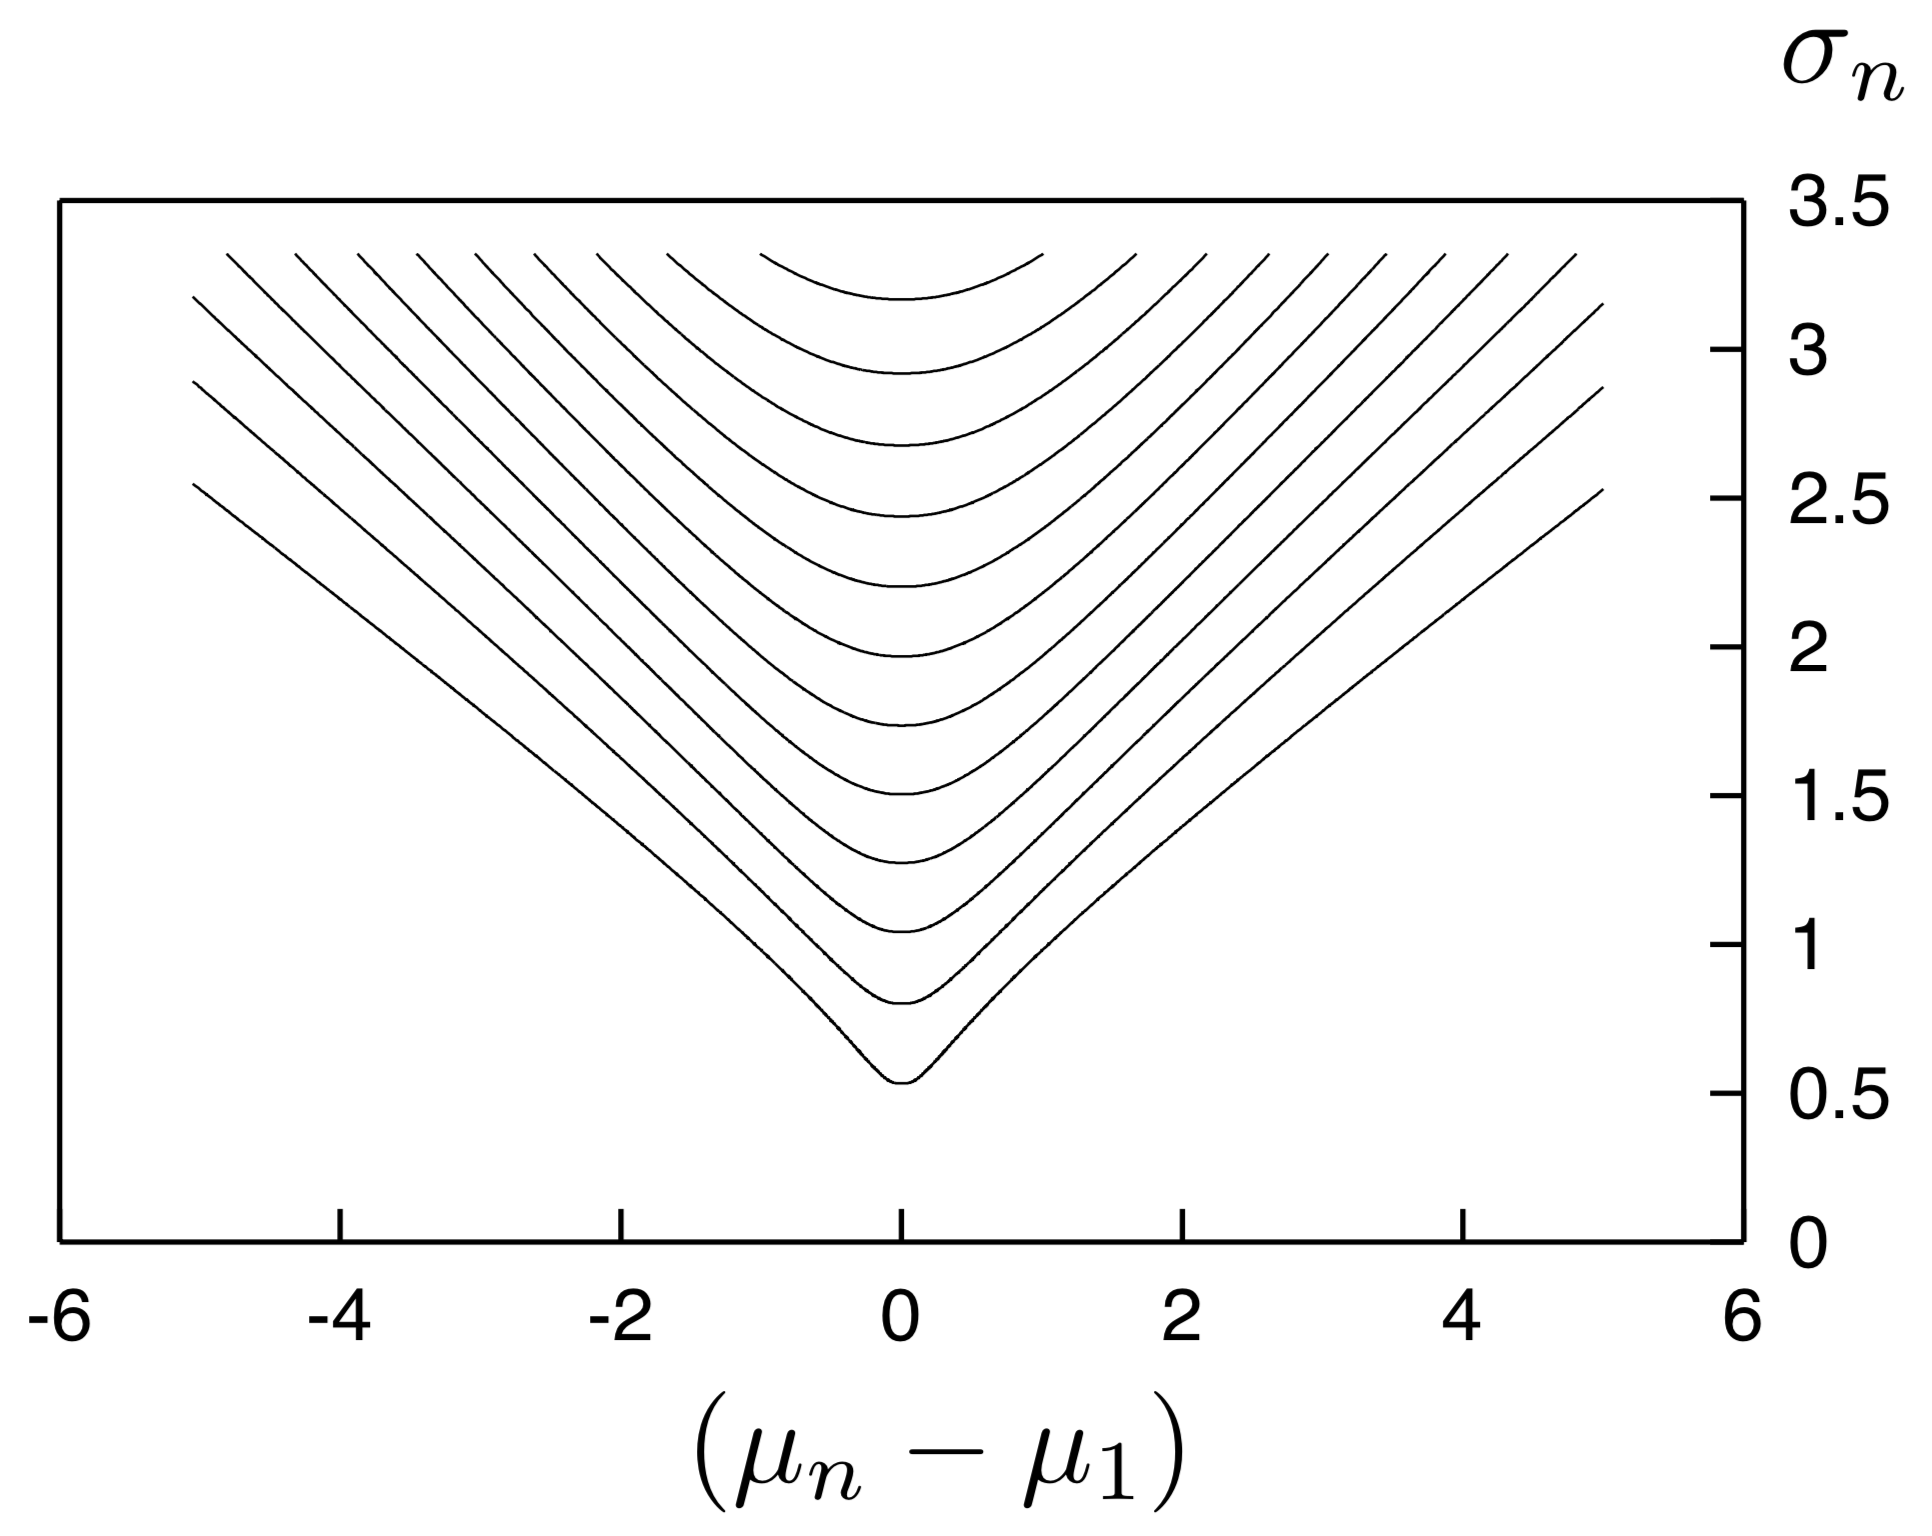
\includegraphics[height=5.5cm]{../slides/figures/exploration-bonus}
\caption{Contour plot for $\Delta_n$, with values increasing towards the top. Reproduced from \citet[ch.~36]{itila}.}
\label{fig:exploration-bonus}
\end{figure}




\subsection{\questionref{q:timing}}
No, in both cases the mining location is fixed \emph{before} observing the data from the prospecting. This means that the utility is not a function of the data. For both cases, the expected utility is
\begin{align}
\Exp{p(\vx)}{U(\vx, p, m)} = \Exp{\vx}{-c_p + x_m} = -c_p + \mu_m
\end{align}
where the answer to the first part of the question has $m = p$.

This shows that the difficulty (and the benefit!) comes from the fact that future decisions are a function of data that will be observed in the future. Because we have beliefs over what this future data will be, we can still take the expectations.




\subsection{\questionref{q:prob-improv}}
First, let's compute the probability that we would actually make a switch based on the data obtained from prospecting. The site we prospect at $p$ is the only one that has a posterior mean $\mu_p'$ which is affected by the data from the prospecting $d_p$. We denote the highest prior mean of all other sites as $\mu_1$ (\cref{eq:highest-other}). In this explanation, we only consider the case that $\mu_1 > \mu_p$, as the opposite case is similar.

Remember \cref{eq:m-given-data}, which states that we choose the site to mine based on the highest posterior mean return given the data. For the case that $\mu_1 > \mu_p$, we will only switch our decision to site $p$ if $\mu_p' > \mu_1$. We calculate the probability of this happening using the same $p(\mu_p')$ as before:
\begin{align}
P(\mu_p' > \mu_1) &= \int_{\mu_1}^\infty p(\mu_p') \calcd{\mu_p'} = \int_{\mu_1}^\infty \NormDist{\mu_p'; \mu_p, \sigma_p^2\frac{\sigma_p^2}{\sigma^2 + \sigma_p^2}} \calcd{\mu_p'} \nonumber \\
&= 1 - \int_{-\infty}^{\mu_1} \NormDist{\mu_p'; \mu_p, \sigma_p^2\frac{\sigma_p^2}{\sigma^2 + \sigma_p^2}} \calcd{\mu_p'} \nonumber \\
&= 1 - \Phi\left(\frac{\mu_1-\mu_p}{\sigma_p^2}\sqrt{\sigma^2 + \sigma^2_p}\right) = 1 - \Phi\left(\frac{\mu_1-\mu_p}{s}\right)  \label{eq:prob-improv} \,,
\end{align}
where
\begin{align}
s^2 = \sigma_p^2\frac{\sigma_p^2}{\sigma^2 + \sigma_p^2} \,, \qquad \text{ and } \qquad \Phi(x) = \int \NormDist{x';, 0, 1} \calcd{x'} \,.
\end{align}
We can compare this to the expected improvement $\Delta_p$ for the case that $\mu_1 > \mu_p$ (from \cref{eq:prospecting-ei}):
\begin{align}
\Delta_p &= -c_p + \int_{\mu_1}^\infty p(\mu_p')\left(\mu_p' - \mu_1\right)\calcd{\mu_p'} \\
&= -c_p + \int_{\mu_1}^\infty \NormDist{\mu_p'; \mu_p, s^2}\left(\mu_p' - \mu_1\right)\calcd{\mu_p'} \,.
\end{align}
Using the equation for the mean of a truncated Gaussian \citep{wiki:trunc-normal}, we can find the solution to the integral (keep in mind that in our integral we do not normalise the truncated Gaussian):
\begin{align}
% \Delta_p &= -c_p + \left(1 - \Phi\left(\frac{\mu_1-\mu_p}{s}\right)\right)\left(\mu_p-\mu_1\right) + \NormDist{\mu_1; \mu_p, s^2}\cdot s \\
\Delta_p &= -c_p + \left(1 - \Phi\left(\frac{\mu_1-\mu_p}{s}\right)\right)\left(\mu_p-\mu_1\right) + \phi\left(\frac{\mu_1 - \mu_p}{s}\right)s \label{eq:explicit-prospecting-ei} \,,
\end{align}
where we write the standard Gaussian density as $\phi(\cdot)$.

We have now computed the probability of improvement (\cref{eq:prob-improv}), as well as the explicit form for the expected improvment (\cref{eq:explicit-prospecting-ei}). We want to
\begin{itemize}
\item see how the probability of improvement changes,
\item for constant expected improvement,
\item as $\mu_p - \mu_1$ increases (and therefore $\sigma_p$ increases as well).
\end{itemize}
Since it is difficult to see how $\sigma_p$ needs to change to keep the expected improvement contant, we instead notice that keeping $(\mu_1 - \mu_p)/s$ constant keeps the probability of improvement constant. This implies
\begin{align}
\frac{\mu_1 - \mu_p}{s} = \frac{(\mu_1 - \mu_p)\sqrt{\sigma^2 + \sigma_p^2}}{\sigma_p^2} = c = \text{const}
\quad \implies \quad
\sigma_p^2 = \frac{\sigma^2 (\mu_1 - \mu_p)^2}{c^2 - (\mu_1 - \mu_p)^2} \,.
\end{align}
By looking at \cref{eq:explicit-prospecting-ei}, we see that for a constant $(\mu_1 -\mu_p)/s$, with increasing $\mu_1 - \mu_p$, the expected improvement monotonically increases. This implies that if we instead keep the expected improvement fixed while increasing $\mu_1 - \mu_p$, then the ratio $(\mu_1 - \mu_p)/s$ would have to decrease.

So to summarise, a large difference in means $\mu_1 - \mu_p$ can still lead to a given expected improvement if $\sigma_p^2$ is large enough. However, for larger gaps in means, the probability that we will see an improvement becomes smaller.




\subsection{\questionref{q:single-obs-bo}}
We are given a Gaussian process posterior for $N$ data points in $(X, \vy)$
\begin{align}
p(f\given \vy, X) = \GP\big( \underbrace{k(\vx, X) k(X, X)\inv \vy}_{\mu'(\vx)}, \quad \underbrace{k(\vx, \vx') - k(\vx, X)k(X, X)\inv k(X, \vx')}_{k'(\vx, \vx')}\big) \,.
\end{align}
Our utility function is
\begin{align}
U(\vx, f) = \max\left\{f(\vx), f(\vx^*)\right\}
\end{align}
where $\vx^*$ is the input location with the best function value that we have seen so far. To find the next place to evaluate, we simply apply next two steps of decision theory: finding the expected utility, and optimising it. We first find the expected utility:
\begin{align}
\Exp{p(f\given\vy, X)}{U(\vx, f)} = \Exp{p(f\given\vy, X)}{\max\left\{f(\vx), f(\vx^*)\right\}} \,.
\end{align}
We know that in a noiseless Gaussian process posterior, the predictive variance is zero for observed points. Since $f(\vx^*)$ is an observed point (contained in the data $\data = (X, \vy)$), it will not be uncertain. Therefore, we only need to take the expectation over the function at the candidate point $\vx$:
\begin{align}
&\Exp{p(f\given\vy, X)}{U(\vx, f)} = \Exp{p(f(\vx)\given\vy, X)}{\max\left\{f(\vx), f(\vx^*)\right\}} \nonumber \\
&= \int_{-\infty}^\infty \NormDist{f(\vx); \mu'(\vx), k(\vx, \vx')} \max\left\{f(\vx), f(\vx^*)\right\} \calcd{f(\vx)} \nonumber \\
&= \int_{-\infty}^{f(\vx^*)} \NormDist{f(\vx); \mu'(\vx), k(\vx, \vx')} f(\vx^*) \calcd{f(\vx)} + \int_{f(\vx^*)}^{\infty} \NormDist{f(\vx); \mu'(\vx), k(\vx, \vx')} f(\vx) \calcd{f(\vx)} \nonumber \\
&= f(\vx^*) \Phi\left(\frac{f(\vx^*) - \mu'(\vx)}{\sqrt{k'(\vx, \vx)}}\right) + \left(1 - \Phi\left(\frac{f(\vx^*) - \mu'(\vx)}{\sqrt{k'(\vx, \vx)}}\right) \right)\mu'(\vx) + \phi\left(\frac{f(\vx^*) - \mu'(\vx)}{\sqrt{k'(\vx, \vx)}}\right) \sqrt{k'(\vx, \vx)} \nonumber \\
&= \mu'(\vx) + \underbrace{\left(f(\vx^*) - \mu'(\vx)\right)\Phi\left(\frac{f(\vx^*) - \mu'(\vx)}{\sqrt{k'(\vx, \vx)}}\right) + \phi\left(\frac{f(\vx^*) - \mu'(\vx)}{\sqrt{k'(\vx, \vx)}}\right) \sqrt{k'(\vx, \vx)}}_{\text{Expected improvement}} \,.
\end{align}
Then we pick the point that has the largest value of the expression above. This can be done through gridding or numerical optimisation.

Notice how we want to pick the point with the highest mean \emph{plus} the expected improvement over the earlier evaluation $f(\vx)$. Simply picking the point with the highest $\mu'(\vx)$ would be what we would do if we did not have any existing evaluations. However, since we can always fall back on our previous evaluation with a reward of $f(\vx)$, decision theory tells us to explore more aggressively.



\subsection{\questionref{q:laplace-gpc}}
This discussion follows \citet[\S 3.4.1]{gpml}, although they use a slightly different likelihood. For completeness, I restate the Laplace approximation for an unnormalised probability distribution $\tilde p(\vf)$
\begin{align}
q(\vf) = \NormDist{\vf; \vf^*, -\nabla^2_\vf\log \tilde p(\vf)\vert_{\vf^*}\inv} \,, \qquad
\vf^* = \argmax_{\vf} \tilde{p}(\vf) \,.
\end{align}
This comes from a second order Taylor series expansion of $\tilde p(\vf)$
\begin{align}
p(\vf) \approx q(\vf) = -\log Z + \underbrace{\nabla_\vf\log \tilde p(\vf)\vert_{\vf^*}}_{=0} (\vf-\vf^*) + \frac{1}{2}(\vf-\vf^*)\transpose\nabla^2_\vf\log \tilde p(\vf)\vert_{\vf^*}(\vf-\vf^*) \,,
\end{align}
which implies a Gaussian approximation.

\subsubsection{Condition at the optimum}
\begin{align}
\nabla_\vf \left[\log p(\vf) + \sum_{n=1}^N \log p(y_n\given f(\vx_n), \vx_n)\right] &= \nabla_\vf \left[-\frac{1}{2}\log 2\pi\detbar{\mat K} - \frac{1}{2}\vf\transpose\mat K\inv\vf + \sum_{n=1}^N \log p(y_n\given f(\vx_n), \vx_n)\right] \nonumber \\
&= - \mat K\inv\vf +  \sum_{n=1}^N\nabla_\vf\log p(y_n\given f(\vx_n), \vx_n) \\
\implies \vf &= \mat K \sum_{n=1}^N\nabla_\vf \log p(y_n\given f(\vx_n), \vx_n)
\end{align}

If you struggle to take first derivatives w.r.t.~vectors, remember that for $f(\vx) \in \Reals\,, \vx\in\Reals^D$ we have
\begin{align}
\nabla_\vx f(\vx)\in \Reals^D \quad\text{with } \left[\nabla_\vx f(\vx)\right]_d = \pderiv[f(\vx)]{x_d} \,.
\end{align}
You can obtain the derivative of any vector-input function by writing it as a sum, and then taking the partial derivative, i.e.~for $f(\vx) = \vx\transpose \mat A\vx$ with symmetric $\mat A$
\begin{align}
\left[\nabla_\vx f(\vx)\right]_d &= \pderiv[]{x_d}\sum_{i=1}^D\sum_{j=1}^D x_{i} A_{ij} x_{j} = \sum_{ij} \left[ \pderiv[x_i]{x_d}A_{ij}x_j + x_iA_{ij}\pderiv[x_j]{x_d} \right] = 2 \sum_{j}A_{dj}x_j \nonumber \\
&= [2\mat A\vx]_d
\end{align}
This uses that $\pderiv[x_i]{x_d}$ is only 1 when $i=d$.

\subsubsection{Covariance of Laplace approximation}
From the definition of the Laplace approximation (you should know this) the covariance is equal to the negative inverse Hessian of the objective function at the optimum. Let's find an expression for the Hessian.
\begin{align}
\nabla_\vf^2 \left[\log p(\vf) + \sum_{n=1}^N \log p(y_n\given f(\vx_n), \vx_n)\right] &= \nabla_\vf^2 \left[-\frac{1}{2}\log 2\pi\detbar{\mat K} - \frac{1}{2}\vf\transpose\mat K\inv\vf + \sum_{n=1}^N \log p(y_n\given f(\vx_n), \vx_n)\right] \nonumber \\
&= \nabla_\vf\left[- \mat K\inv\vf + \sum_{n=1}^N\nabla_\vf \log p(y_n\given f(\vx_n), \vx_n)\right] \nonumber \\
&= -\mat K\inv + \sum_{n=1}^N \nabla_\vf^2\log p(y_n\given f(\vx_n), \vx_n) \nonumber \\
&= -\mat K\inv - \mat W \nonumber
\end{align}
Here $\mat W$ is diagonal with $W_{nn} = \nabla_{f(\vx_n)}^2\log p(y_n\given f(\vx_n), \vx_n)$, as each likelihood term only depends on a single element in $\vf$, i.e.~$f(\vx_n)$. To be completely explicit, one should actually compute the terms $W_{nn}$, but this is standard, as it is simply differentiation w.r.t.~one variable.

\subsubsection{Clearly state the approximation}
So, overall we get the approximation
\begin{align}
q(\vf) = \NormDist{\vf; \vf^*, (\mat K\inv + \mat W)\inv} \,.
\end{align}

\subsubsection{Monte Carlo approximation}
Remember that we denoted $\vf = f(X)$.
\begin{align}
p^* = p(y^*\given \vx^*, \vy, X) &= \int p(y^*\given f(\vx^*), \vx^*) p(f(\vx^*), f(X)\given \vx^*, \vy, X) \calcd{f(\vx^*)} \calcd{f(X)} \\
&=\int p(y^*\given f(\vx^*), \vx^*) p(f(\vx^*)\given f(X), X, \vx^*) p(f(X)\given \vy, X)  \calcd{f(X)} \calcd{f(\vx^*)} \\
&\approx \int p(y^*\given f(\vx^*), \vx^*) \left[\int p(f(\vx^*)\given f(X), X, \vx^*) q(f(X))  \calcd{f(X)} \right] \calcd{f(\vx^*)}
\end{align}
The inner integral can be performed using the standard Gaussian manipulations, to get
\begin{align}
q(f(\vx^*)) &= \int p(f(\vx^*)\given f(X), X, \vx^*) q(f(X))  \calcd{f(X)} \\
&= \mathcal N \Big(f(\vx^*); k(\vx^*, X)\mat K\inv\vf^*, \\
& \quad \qquad k(\vx^*,\vx^*) - k(\vx^*, X)\mat K\inv\left[\mat K - (\mat K\inv + \mat W)\inv\right]\mat K\inv k(X, \vx^*)\Big) \,.
\end{align}
You should be able to derive this. The trick is to note that
\begin{gather}
f(\vx^*) = k(\vx^*, X)\mat K\inv\vf + \epsilon \,, \\
\vf \sim q(\vf) \,, \qquad \epsilon \sim \NormDist{0, k(\vx^*, \vx^*) - k(\vx^*, X)\mat K\inv k(X, \vx^*)} \,.
\end{gather}

The Monte Carlo estimate becomes
\begin{align}
\hat p^* = \frac{1}{S}\sum_{s=1}^S p(y^*\given f(\vx^*) = f^{(s)}, \vx^*) \,,  && f^{(s)} \overset{iid}{\sim} q(f(\vx^*)) \,.
\end{align}


\subsubsection{Monte Carlo approximation: Alternative}
Todo, ask about this in lectures. You can also sample from $q(f(X))$, rather than doing he integral in closed-form.

\subsection{\questionref{q:laplace-gpr}}
Following the same procedure as in the previous question, we find the mean and covariance for the Laplace approximation.
\begin{align}
\log p(\vf\given\vy, X) &= \text{const} + -\frac{1}{2}\vf\transpose\mat K\inv\vf - \frac{1}{2}(\vf - \vy)\transpose\mat \Sigma\inv(\vf-\vy) \\
&= \text{const} + -\frac{1}{2}\vf\transpose\mat K\inv\vf - \frac{1}{2}\vf\transpose\mat \Sigma\inv\vf + \vf\transpose\mat\Sigma\inv\vy -\frac{1}{2}\vy\transpose\mat\Sigma\inv\vy
%(\vf - \vy)\transpose\mat \Sigma\inv(\vf-\vy)
\end{align}
\begin{align}
\nabla_\vf \log p(\vf\given\vy,X) &= -\mat K\inv\vf - \mat\Sigma\inv\vf + \mat\Sigma\inv\vy = 0 \\
\implies \vf^* &= (\mat K\inv + \mat\Sigma\inv)\inv\mat\Sigma\inv\vy \\
&= \mat K(\mat K + \mat\Sigma)\inv\vy
\end{align}
\begin{align}
\nabla_\vf^2 \log p(\vf\given\vy,X)&= -\mat K\inv - \mat\Sigma\inv = -(\mat K\inv +\mat\Sigma\inv) \\
\implies q(\vf) &= \NormDist{\vf; \mat K(\mat K+\mat\Sigma)\inv\vy, (\mat K\inv + \mat\Sigma\inv)\inv}
\end{align}
We can apply Woodbury to get this into a more familiar form...
\begin{align}
q(\vf) = \NormDist{\vf; \mat K(\mat K+\mat\Sigma)\inv\vy, \mat K - \mat K(\mat K + \mat\Sigma)\inv\mat K}
\end{align}
This looks familiar.

\subsection{\questionref{q:rejection-sampling-proof}}
Lecture.

\subsection{\questionref{q:importance-sampling-unnormalised}}
Lecture.

\subsection{\questionref{q:importance-sampling-variance}}
Lecture.

\subsection{\questionref{q:hyperparam-non-conjugate-gp-likelihoods}}
 \subsubsection{State the integral for $p(y^*|\vy)$ for a GP}
 We can write this as
 \begin{align}
     p(y^*|\vy) &= \int \int \int p( y^* | f^* ) p( f^* | \vf, \vtheta ) p( \vf, \vtheta | \vy ) \calcd f^* \calcd \vtheta \calcd \vf. \label{eq:hyperparam-non-conjugate-gp-integral}
 \end{align}

 \subsubsection{State the Monte Carlo approximation to this integral}
 We can write the above integral in terms of expectations
 \begin{align}
     p( y^* | \vy) = \Exp{p( \vf, \vtheta | \vy )}{ \Exp{p( f^* | \vf, \vtheta )}{p( y^* | f^* ) }}.
 \end{align}
 The inner expectation over $p( f^* | \vf, \vtheta )$ is intractable in general (for a non-conjugate likelihood $p( y^* | f^* )$). Similarly the posterior $p( \vf | \vy )$ cannot be found in closed form for a general likelihood, and the hyperparameter posterior $p( \vtheta | \vy)$ is usually intractable even if the likelihood is Gaussian (see~\questionref{q:gp-hyper-conj}). Thus the joint posterior $p( \vf, \vtheta | \vy )$ is intractable, as is its expectation.

 Given these intractabilities, we resort to the following Monte Carlo approximation
 \begin{align}
     p( y^* | \vy) = \frac{1}{K} \sum_k^K \ p( y^* | f^{*(k)} ), \quad f^{*(k)} \sim p( f^* | \vf^{(k)}, \vtheta^{(k)} ), \quad \vtheta^{(k)}, \vf^{(k)} \sim p( \vf, \vtheta | \vy ).\label{eq:hyperparam-non-conjugate-gp-mc}
 \end{align}


 \subsubsection{State the procedure for computing samples for the Monte Carlo approximation}
 We need to draw samples from  $p( \vf, \vtheta | \vy )$ and $p( f^* | \vf, \vtheta )$. While $p( \vf, \vtheta | \vy )$ is intractable, we can sample using the Metropolis algorithm (or another MCMC algorithm). We would target the tractable joint density
 \begin{align}
 p( \vf, \vtheta, \vy ) = p( \vy | \vf ) p( \vf | \vtheta ) p( \vtheta )
 \end{align}
 where $p(\vtheta)$ is prior on hyperparameters. This is justified as $p( \vf, \vtheta, \vy )$ is proportional to the joint posterior $p( \vf, \vtheta | \vy )$ (w.r.t $\vtheta$ and $\vf$). Note that $\vy$ is the observed data and so is fixed in our target density.

 For our sampler, we could use a symmetric proposal $\hat{T}( \vs' | \vs^{(t)} ) = \NormDist{\vs^{(t)}, \mat\Sigma}$ where state $\vs=[\vf\transpose, \vtheta\transpose, \vy\transpose]\transpose$. $\mat\Sigma$ could diagonal, but we could improve sampling efficiency by choosing the submatrix $\mat\Sigma_\vf$ to reflect the covariance of the GP on $\vf$. As $\hat{T}( \vs' | \vs^{(t)} )=\hat{T}( \vs^{(t)} | \vs' )$, the proposal densities cancel out in the acceptance probability which reduces to $p( \vs' ) / p( \vs^{(t)} )$.

 After sampling $\vf^{(t)}, \vtheta^{(t)}$, we can compute $p( f^{*} | \vf^{(t)}, \vtheta^{(t)} )$ analytically (Gaussian conditioning), and then sample from the resulting multivariate Gaussian.

\subsection{\questionref{q:independent-chains}}

Consider two independent Markov chains generated by a transition operator $T$ such that $p(\vx^{(t+1)}|\vx^{(1)},\cdots, \vx^{(t)}) = T(\vx^{(t+1)}|\vx^{(t)})$, and denote the samples from chain $i \in \{1,2\}$ at time $t$ as $x_i^{(t)}$.
The question asks us to show independence between $x_1^{(\tau)}$ and $x_2^{(\tau)}$ where $\tau$ refers to the timestep of the final states mentioned in the question.

Consider the joint $p(\vx_1^{(\tau)}, \vx_2^{(\tau)})$. The way the samples from this distribution are drawn is by applying the transition operator $T$ independently to the previous samples $\vx_1^{(\tau-1)}$ and $\vx_2^{(\tau-1)}$. Therefore, we have
\begin{align}
p(\vx_1^{(\tau)}, \vx_2^{(\tau)}) &= p(\vx_1^{(\tau)}, \vx_2^{(\tau)}|\vx_1^{(\tau-1)}, \vx_2^{(\tau-1)}) p(\vx_1^{(\tau-1)}, \vx_2^{(\tau-1)}) \\
&= T(\vx_1^{(\tau)}|\vx_1^{(\tau-1)})T( \vx_2^{(\tau)}|\vx_2^{(\tau-1)}) p(\vx_1^{(\tau-1)}, \vx_2^{(\tau-1)}) \\
& \cdots \\
&= \prod_{t=1}^{\tau} T(\vx_1^{(t)}|\vx_1^{(t-1)})T( \vx_2^{(t)}|\vx_2^{(t-1)}) p(\vx_1^{(0)}, \vx_2^{(0)})
\end{align}
after propagating the effect of the transition operator for each of the $\tau$ steps. Since the Markov chains are initialised independently, we can take the initial states as chosen independently at random from some identical distribution $p(\vx^{(0)})$. The joint starting distribution will therefore factorise as $p(\vx_1^{(0)}, \vx_2^{(0)}) = p(\vx_1^{(0)}) p(\vx_2^{(0)}) $. Hence we can write
\begin{align}
p(\vx_1^{(\tau)}, \vx_2^{(\tau)}) &=  \prod_{t=1}^{\tau} T(\vx_1^{(t)}|\vx_1^{(t-1)})T( \vx_2^{(t)}|\vx_2^{(t-1)}) p(\vx_1^{(0)}) p(\vx_2^{(0)}) \\
 &=  \left(\prod_{t=1}^{\tau} T(\vx_1^{(t)}|\vx_1^{(t-1)})p(\vx_1^{(0)})\right)\left(\prod_{t=1}^{\tau} T(\vx_2^{(t)}|\vx_2^{(t-1)})p(\vx_2^{(0)})\right) \\
& = p(\vx_1^{(\tau)})p(\vx_2^{(\tau)}),
\end{align}
and the joint factors into two terms $p(\vx_i^{(\tau)})=\prod_{t=1}^{\tau} T(\vx_i^{(t)}|\vx_i^{(t-1)}) p(\vx_i^{(0)})$, and we conclude that the samples from the Markov chains at time $\tau$ are independent.

\subsection{\questionref{q:gradients}}
You should be able to derive a variational lower bound, which for this model becomes:
\begin{align}
\lb = \sum_{n=1}^N\Exp{q(f(X))}{\log p(\vy\given f(\vx_n), \vx_n)} - \KL{q(f(X))}{p(f(X))}
\end{align}
For the reparameterisation gradient, we first rewrite the expected log-likelihood term as
\begin{align}
\Exp{q(f(X))}{\log p(\vy\given f(\vx_n), \vx_n)} &= \Exp{q(f(\vx_n))}{y_n\log [\sigma(f(\vx_n))] + (1-y_n)\log[1-\sigma(f(\vx_n)])} \\
&= \Exp{q(\epsilon)}{y_n\log [\sigma(\mu_n + \sigma_n\epsilon)] + (1-y_n)\log[1-\sigma(\mu_n + \sigma_n\epsilon)])} \,,
\end{align}
where $\mu_n$ and $\sigma_n$ are the mean and stddev of $q(f(\vx_n))$. Some crucial observations:
\begin{itemize}
\item We only need to sample 1D Gaussians, since each term in the expected log-likelihood depends only on the marginal of $q(f(X))$, $q(f(\vx_n))$.
\item We still get a tighter bound by parameterising $q(f(X))$ as a full-rank Gaussian, i.e.~$q(f(X)) = \NormDist{f(X), \vmu, \mat\Sigma}$, since the KL divergence depends on the correlations.
\end{itemize}

Now we develop an expression for the reparameterisation gradient estimator of one term in the sum. The final estimator will be a sum over a minibatch of points. We start with a general expression for the reparameterisation gradient. Note that since the KL divergence can be computed in closed-form, I will not include it in the derivation, as it just requires differentiation of a computable quantity.
\begin{align}
\nabla_\mu\Exp{q(\epsilon)}{\log p(y_n\given f(\vx)= \mu + \sigma\epsilon, \vx)} &= \Exp{q(\epsilon)}{\nabla_{f(\vx)}\log p(y_n\given f(\vx), \vx)\vert_{f(\vx) = \mu+\sigma\epsilon}\cdot\nabla_{\mu}(\mu+\sigma\epsilon)} \\
&=\Exp{q(\epsilon)}{\nabla_{f(\vx)}\log p(y_n\given f(\vx), \vx)\vert_{f(\vx) = \mu+\sigma\epsilon}} \\
\nabla_\sigma\Exp{q(\epsilon)}{\log p(y_n\given f(\vx)= \mu + \sigma\epsilon, \vx)} &= \Exp{q(\epsilon)}{\nabla_{f(\vx)}\log p(y_n\given f(\vx), \vx)\vert_{f(\vx) = \mu+\sigma\epsilon}\cdot\epsilon}% \\
%\nabla_{f(\vx)}\log p(y_n\given f(\vx), \vx) &= 
\end{align}
The Monte Carlo estimator can be found simply by sampling from $q(\epsilon)$.

This is roughly the level of detail you would need to do on the exam. Write out the chain rule until you get to the reparameterisation of the variational distribution. Intermediate terms like 
\begin{align}
\nabla_{f(\vx)}\log p(y_n\given f(\vx), \vx) \vert_{f(\vx) = \mu+\sigma\epsilon}
\end{align}
 do not have to be differentiated unless asked explicitly.

\subsection{\questionref{q:bnn}}
A neural network is a function that is parameterised through weights $\vw$. So we write the neural network as $f(\vx; \vw)$. We assume a general likelihood which depends only on the output for a single input, i.e.~$p(y_n\given f(\vx_n; \vw))$, and a Gaussian prior on the weights $p(\vw) = \NormDist{\vw; 0, \lambda\inv}$.
The variational lower bound becomes
\begin{align}
\lb = \sumn\Exp{q(\vw)}{\log p(y_n\given f(\vx; \vw))} - \KL{q(\vw)}{p(\vw)} \,.
\end{align}
We assume a mean-field variational distribution $q(\vw) = \prod_{i}\NormDist{w_i; \mu_i, \sigma_i^2}$.

In the previous question, each likelihood term depended only on a single variational distribution. In this question, we need to sample \emph{all} the weights. We write our reparameterisation trick as
\begin{align}
\vw = \vmu + \boldsymbol{\sigma} \circ \vepsilon 
\end{align}
where $\circ$ denotes elementwise multiplication. Now we can write the gradients as
\begin{align}
\nabla_{\boldsymbol{\mu}}\Exp{q(\vepsilon)}{\log p(y_n\given f(\vx;\vw))} &= \Exp{q(\vepsilon)}{\nabla_{f(\vx; \vw)}\!\log p(y_n\given f(\vx; \vw))\vert_{\vw=\vmu+\boldsymbol{\sigma}\vepsilon}\nabla_{\vw}f(\vx;\vw)\vert_{\vw=\vmu+\boldsymbol\sigma\vepsilon}} \\
\nabla_{\boldsymbol{\sigma}}\Exp{q(\vepsilon)}{\log p(y_n\given f(\vx;\vw))} &= \Exp{q(\vepsilon)}{\nabla_{f(\vx; \vw)}\!\log p(y_n\given f(\vx; \vw))\vert_{\vw=\vmu+\boldsymbol\sigma\vepsilon}\nabla_{\vw}f(\vx;\vw)\vert_{\vw=\vmu+\boldsymbol\sigma\vepsilon} \circ \boldsymbol\vepsilon}
\end{align}
and find Monte Carlo estimates in the usual way. Note that we again apply the chain rule until we differentiate through the reparameterisation.


\subsection{\questionref{q:vae}}
For a single data point we have the ELBO
\begin{align}
\lb_n = \Exp{q(\vz_n)}{\log p(\vx_n\given\vz_n; \theta)} - \KL{q(\vz_n)}{p(\vx_n)} \,.
\end{align}
The approximate posterior is parameterised through a recognition network with parameters $\phi$, so we denote
\begin{align}
q(\vx_n; \phi) = \NormDist{\vx_n; \vmu(\vx_n, \phi), \mathbf \Sigma(\vx_n, \phi)} \,.
\end{align}
Writing using the reparamterisation trick
\begin{align}
\lb_n = \Exp{q(\vepsilon)}{\log p(\vx_n; \vz_n=\vmu(\vx_n, \phi) + \mathbf\Sigma(\vx_n, \phi)^{\frac{1}{2}}\vepsilon)} - \mathrm{KL} \,.
\end{align}
We can now take gradients. We start with the gradient of the model parameters $\theta$
\begin{align}
\nabla_\theta\lb_n = \Exp{q(\vepsilon)}{\nabla_{\bar\vx_n} \log \NormDist{\vx_n; \bar\vx_n, \sigma^2}\vert_{\bar\vx_n = f_\theta(\vz_n)}\nabla_{\theta}f_\theta(\vz_n=\vmu\dots)} \,.
\end{align}
Similar for the parameters of the inference network $\phi$.









\printbibliography

\end{document}